%Shared
% Exemplo LaTeX de monografia UCS
%
% Elaborado com base nas orientações dadas no documento
% ``GUIA PARA ELABORAÇÃO DE TRABALHOS ACADÊMICOS''
% disponível no site da biblioteca da Unisinos.
% http://www.unisinos.br/biblioteca
%
% Os elementos textuais abaixo são apresentados na ordem em que devem
% aparecer no documento.  Repare que nem todos são obrigatórios - isso
% é devidamente indicado em cada caso.
% 
% Comentários abaixo colocados entre aspas (`` '') foram
% extraídos diretamente do documento da biblioteca.
%
% Este documento é de domínio público.
%
%\begin{figure}[!htb]
%	\caption{Exemplo de quantização e amostragem}
%	\label{fig:ex_quant_amos_img}
%	\centering
%	\begin{minipage}{.8\textwidth}
%   \centering
%		\includegraphics[width=.5\textwidth]{Figuras/ex_quant_amos_img.jpg}
%		\fonte{\cite{Zibetti03}.}
%	\end{minipage}
%\end{figure}

%=======================================================================
% Declarações iniciais identificando a classe de documento e
% selecionando alguns pacotes adicionais.
%
% As opções disponíveis (separe-as com vírgulas, sem espaço) são:
% - twoside: Formata o documento para impressão frente-e-verso
%   (o default é somente-frente)
% - english,brazilian,french,german,etc.: idiomas usados no documento.
%   Deve ser colocado por último o idioma principal.
%=======================================================================

\documentclass[oneside,english,brazilian]{UCSmonografia}
\usepackage[utf8]{inputenc} % charset do texto (utf8, latin1, etc.)
\usepackage[T1]{fontenc} % encoding da fonte (afeta a sep. de sílabas)
\usepackage{graphicx} % comandos para gráficos e inclusão de figuras
\usepackage[export]{adjustbox}
\usepackage{bibentry} % para inserir refs. bib. no meio do texto
\usepackage{algpseudocode}
\usepackage{algorithm}
\usepackage{amsmath}
\usepackage{amssymb}
\usepackage{amsthm}
\usepackage{mathtools}
\usepackage[section]{placeins}
\usepackage{multirow}
\usepackage{appendix}
\usepackage[autostyle]{csquotes}
\usepackage{xcolor}
\usepackage{enumitem}
\usepackage{setspace}
\usepackage{adjustbox}
\usepackage[graphicx]{realboxes}
\usepackage{url}
\usepackage{subfigure}

\usepackage{listings}
\onehalfspacing

\usepackage{textcase}
\usepackage{etoolbox}

\urlstyle{same}

\makeatletter
\patchcmd{\l@section}{#1}{\MakeTextUppercase{#1}}{}{}
\makeatother


% Definindo novas cores
\definecolor{verde}{rgb}{0.25,0.5,0.35}
\definecolor{jpurple}{rgb}{0.5,0,0.35}
\definecolor{darkgreen}{rgb}{0.0, 0.2, 0.13}

\newcommand\MyBox[1]{%
  \fbox{\parbox[c][1.7cm][c]{1.7cm}{\centering #1}}%
}
\newcommand\MyVBox[1]{%
  \parbox[c][1.7cm][c]{1cm}{\centering\bfseries #1}%
}  
\newcommand\MyHBox[2][\dimexpr1.7cm+2\fboxsep\relax]{%
  \parbox[c][1cm][c]{#1}{\centering\bfseries #2}%
}  
\newcommand\MyTBox[3]{%
  \MyVBox{#1}
  \MyBox{#2}\hspace*{-\fboxrule}%
  \MyBox{#3}\hspace*{-\fboxrule}%

}

\usepackage{listings}
\onehalfspacing

\newcommand{\estiloJava}{
\lstset{
    language=Java,
    basicstyle=\ttfamily\small,
    keywordstyle=\color{jpurple}\bfseries,
    stringstyle=\color{red},
    commentstyle=\color{verde},
    morecomment=[s][\color{blue}]{/**}{*/},
    extendedchars=true,
    showspaces=false,
    showstringspaces=false,
    numbers=left,
    numberstyle=\tiny,
    breaklines=true,    
    breakautoindent=true,
    captionpos=b,
    xleftmargin=0pt,
    tabsize=2
}}
%\usepackage[portuguese]{babel}


\newtheorem{theorem}{Teorema}[chapter]
\newtheorem{corollary}[theorem]{Corolário}
\newtheorem{lemma}{Lema}[chapter]
\newtheorem{definition}{Definição}[chapter]
\newtheorem{example}{Exemplo}[chapter]
\newtheorem{remark}{Comentário}

%=======================================================================
% Escolha do sistema para geração de referências bibliográficas.
%
% O default é usar o estilo abnt.bst.  Comente a definição abaixo
% e descomente a linha seguinte para usar o estilo do ABNTeX (é
% necessário ter esse pacote instalado).
%
% A vantagem do abnt.bst é que ele permite o uso de um arquivo .bib
% seguindo as orientações tradicionais do BibTeX (veja essas orientações
% em http://ctan.tug.org/tex-archive/biblio/bibtex/contrib/doc/btxdoc.pdf).
% Entretanto, o estilo não suporta algumas citações mais exóticas como
% apud.  Para isso, use o ABNTeX, mas esteja ciente de que muitas de
% suas referências serão incompatíveis com os estilos tradicionais do
% BibTeX como plain, alpha, ieeetr, entre outros.
%=======================================================================
\abntbst
%\usepackage[alf]{abntcite}
%\usepackage[alf]{abntex2cite}
%=======================================================================
% Dados gerais sobre o trabalho.
%=======================================================================
%=======================================================================
% Dados gerais sobre o trabalho.
%=======================================================================
\autor{DANIEL MORAIS}{ERICH}
\titulo{Um estudo sobre modelos cilíndricos para registro de imagens}


%\subtitulo{Versão \LaTeX}
\orientador [Prof. Dr.]{Holsbach Costa}{Guilherme}
%\coorientador[Prof.~Dr.]{Lamport}{Leslie}
\local{Caxias do Sul}
\ano{2020}

%% dados específicos para Dissertação de Mestrado
%% dados da ficha catalográfica (obrigatória somente para diss. e tese)
%cip{Dissertação (mestrado)}{004.732}
%\bibliotecario{Bibliotecária responsável: Fulana da Silva}{12/3456}

%% dados específicos para Dissertação de Mestrado
%% dados da ficha catalográfica (obrigatória somente para diss. e tese)
\cip{Trabalho de Conclusão de Curso}{004.732}
%\bibliotecario{Bibliotecária responsável: Fulana da Silva}{12/3456}

%% dados específicos para monografia de Graduação
\unidade{}
\curso{}
\natureza{%
Trabalho de Conclusão de Curso apresentado como requisito parcial à obtenção do título de Bacharel em Engenharia de Computação na Área do Conhecimento de Ciências Exatas e Engenharias da Universidade de Caxias do Sul
}


%% dados específicos para monografia de Graduação

\natureza{%
Trabalho de Conclusão de Curso apresentado como requisito parcial à obtenção do título de Bacharel em Engenharia de Computação na Área do Conhecimento de Ciências Exatas e Engenharias da Universidade de Caxias do Sul
}
%=======================================================================
% Dados gerais sobre o trabalho.
%=======================================================================
%======================================================================
% Palavra-Chave
%======================================================================

%======================================================================
% Palavra-Chave
%======================================================================
% cada palavra-chave deve ser fornecida duas vezes, uma em português e
% outra no idioma estrangeiro (na verdade, em tantos idiomas quantos se
% desejar).
\palavrachave{brazilian}{Inspetores de rótulos. Imagem panorâmica. Mosaico de imagens. Registro de imagens}
\palavrachave{english}{Label inspectors. Panoramic image. Image mosaic. Image registration}

%======================================================================
% Palavra-Chave
%======================================================================
%=======================================================================
% Início do documento.
%=======================================================================
\everymath{\displaystyle}
\begin{document}
\capa
\folhaderosto
\folhadeaprovacao 
%=======================================================================
%Dedicatória (opcional).
%Agradecimentos (opcional).
%Epígrafe (opcional).
%=======================================================================
%=======================================================================
%Dedicatória (opcional).
%Agradecimentos (opcional).
%Epígrafe (opcional).
%=======================================================================
% Dedicatória (opcional).
%
% O texto é normalmente colocado na parte de baixo da página, alinhado
% à direita.  Mas a formatação é basicamente livre.  Só não se escreve
% a palavra 'dedicatória'.
%=======================================================================
% \begin{dedicatoria}

% \end{dedicatoria}

%=======================================================================
% Agradecimentos (opcional).
%=======================================================================
   \begin{agradecimentos}
    Ao meu orientador, Guilherme H. Costa, pela total dedicação, compreensão e comprometimento em me auxiliar não só no desenvolvimento deste trabalho, mas também em meio a vida acadêmica. Obrigado por me ensinar a trilhar o caminho mais recompensador, no qual exige total comprometimento na execução das tarefas realizadas.
    
    Aos meus professores e orientadores de iniciação científica, pela paciência e por nunca terem se recusado a ajudar, mesmo quando não lhes era conveniente.
    
    Aos amigos Anderson, Matheus Nathan, Thiago, Douglas e Mateus Gaspary que trilharam o caminho da graduação ao meu lado, compartilhando conhecimentos e ajudando-me a superar novos desafios constantemente. Um agradecimento especial a Iuri Crestani e Rodrigo Dallagnol, que do primeiro ao último dia da graduação, fizeram a árdua caminhada valer muito mais a pena.
    
    Aos amigos de longa data João Paulo Guedes, Emiliano Piazer e Lucas Matos por sempre estarem ao meu lado, mesmo nos momentos mais difíceis. Um destaque a Alexsandro Gabrielli que teve influência direta na minha escolha profissional.
    
    Aos meus familiares Halisson, Gustavo, Juarez e Deonice que sempre fizeram o possível e o impossível para que eu concluísse o curso, me motivando a seguir em frente perante todas as dificuldades. Espero imensamente poder retribuir tudo que foi feito por vocês durante esse período, sem o apoio e incentivo prestados por vocês, nada disso teria sido possível.
    
    E por fim, a todos que direta ou indiretamente fizeram parte da minha formação, o meu
    muito obrigado.
   \end{agradecimentos}

%=======================================================================
% Epígrafe (opcional).
%
% ``[...] o autor apresenta uma citação, seguida de indicação de autoria,
% relacionada com a matéria tratada no corpo do trabalho. Podem, também,
% constar epígrafes nas folhas de aberturas das seções primárias.''
%=======================================================================
\begin{epigrafe}
  		``\textit{To get what you want, you must look beyond what you see.}''
  		
  		
Rafiki, The Lion King
\end{epigrafe}
%=======================================================================
%Dedicatória (opcional).
%Agradecimentos (opcional).
%Epígrafe (opcional).
%=======================================================================
%=======================================================================
% Resumo 
%=======================================================================
%=======================================================================
% Resumo em Português. 
%O resumo deve ressaltar o objetivo, o método, os resultados e as conclusões do documento. A ordem e a extensão destes itens dependem do tipo de resumo (informativo ou indicativo) e do tratamento que cada item recebe no documento original. O resumo deve ser precedido da referência do documento, com exceção do resumo inserido no próprio documento.
% A recomendação é para 150 a 500 palavras.
%=======================================================================

\begin{abstract}
\noindent 
Na indústria de envase de bebidas é comum a demanda por sistemas de visão computacional chamados de inspetores de rótulos. Esses sistemas verificam o posicionamento dos rótulos afixados em garrafas, permitindo a retirada automática das garrafas que estejam fora dos padrões de qualidade. Entretanto, os inspetores comerciais  são importados, possuem alto custo, e, aparentemente, se baseiam em reconhecimento de padrões, requerendo novo treinamento para cada novo modelo de garrafa ou rótulo. Uma possibilidade de solução para verificação do posicionamento dos rótulos é uma abordagem baseada no registro de imagens e na correlação entre imagens. Para tanto, como etapa de pré-processamento, pode-se construir uma imagem panorâmica da superfície das garrafas. Visto isso, neste trabalho é proposto o estudo de uma solução para geração de imagens panorâmicas da superfície de objetos cilíndricos.
\end{abstract}

%=======================================================================
% Resumo em língua estrangeira (obrigatório somente para teses e
% dissertações).
%
% O idioma usado aqui deve necessariamente aparecer nos parâmetros do
% \documentclass, no início do documento.
%=======================================================================
\begin{otherlanguage}{english}
\begin{abstract}
\noindent 
In the beverage filling industry, demand for computer vision systems called label inspectors is common. These systems check the positioning of the labels affixed to the bottles, allowing the automatic removal of bottles that are outside the quality standards. However, commercial inspectors are imported, expensive and seemingly based on pattern recognition, requiring new training for each new bottle or label model. A possible solution to check the positioning of the labels is an approach based on the registration of images and the correlation between images. For this, as a pre-processing step, a panoramic image of the bottles' surface can be constructed. In view of this, this work proposes the study of a solution to generate panoramic images of the surface of cylindrical objects.
\end{abstract}
\end{otherlanguage}

% %=======================================================================
% % Lista de Figuras (opcional).
% %=======================================================================
\listoffigures
% %=======================================================================
% % Lista de Tabelas (opcional).
% %=======================================================================
% \listoftables
%=======================================================================
% Lista de Abreviaturas (opcional).
%
% Relação alfabética das abreviaturas utilizadas no texto,
% seguidas das palavras ou expressões grafadas por extenso.
%=======================================================================
%\begin{listadeabreviaturas}{seg., segs.}
%\item[atual.] atualizado, -a
%\item[coord.] coordenador
%\item[seg., segs.] seguinte, -s
%\end{listadeabreviaturas}

%=======================================================================
% Lista de Siglas (opcional).
%=======================================================================
% %=======================================================================
% % Lista de Siglas (opcional).
% %=======================================================================
% % Apresentadas em ordem alfabética.
% % A sigla, quando aparecer pela primeira vez no texto, deve ser colocada
% % entre parênteses, precedida da forma completa.
% %=======================================================================
% \begin{listadesiglas}{UCS}
% %A
% \item[AP]       \textit{Access Point} (Ponto de Acesso)
% \item[AAHA]     \textit{American Animal Hospital Association}
% %\item[A]       Ampére
% \item[ADC]      \textit{Analog to Digital Converter}
% %\item[ABNT]    \textbf{A}ssociação \textbf{B}rasileira de \textbf{N}ormas \textbf{T}écnicas
% %B
% %\item[BNDES]	\textbf{B}anco \textbf{N}acional do \textbf{Des}envolvimento
% %C
% \item[CPU]      \textit{Central Processing Unit} (Unidade Central de Processamento)
% \item[CI]       Circuito Integrado
% %\item[CISC]     \textit{Complex Instruction Set Computer}
% %\item[CoAP]	\textbf{Co}nstrained \textbf{A}pplication \textbf{P}rotocol
% \item[CA]       Corrente Alternada
% \item[CC]       Corrente Contínua
% %D
% \item[DM2]      Diabetes Mellitus tipo 2
% \item[DAC]      \textit{Digital to Analog Converter}
% %E
% \item[EB]       Energia Bruta
% \item[EM]       Energia Metabolizável
% \item[E/S]      Entrada/Saída
% \item[ECC]      Escore de Condição Corporal
% %F
% %G
% %H
% %\item[HD]       \textit{High Definition}
% %\item[HDMI]    \textbf{H}igh-\textbf{D}efinition \textbf{M}ultimidia \textbf{I}nterface \textbf{E}ngineers
% %I
% \item[I/O]      \textit{Imput/Output}
% %\item[ITEC]     Incubadora Tecnológica de Caxias do Sul
% \item[IP]       \textit{Internetworking Protocol}
% \item[IoT]		\textit{Internet of Things} (Internet das Coisas)
% %\item[IP]		Internet Protocol
% %\item[IPv6]	\textit{Internet Protocol version} 6
% %\item[ICES]		Instituição Comunitária de Educação Superior 
% %\item[IEEE]	Institute of Electrical and Electronics
% %J
% %L
% \item[LHF]      Lipidose Hepática Felina
% %\item[LCD]      \textit{Liquid Crystal Display}
% \item[LAN]      \textit{Local Area Network}
% %M
% \item[M2M]		\textit{Machine to Machine}
% %\item[M2P]		Machine-to-People
% %\item[MP]      Mega Pixels
% %\item[MQTT]	Message Queue Telemetric Transport
% \item[MCU]      Microcontrolador
% %N
% %\item[NFC]		\textbf{N}ear \textbf{F}ield \textbf{C}ommunication
% \item[NE]      Necessidade Energética
% %O
% \item[OSI]      \textit{Open System Interconnection}
% %\item[ONU]		\textbf{O}rganização das \textbf{N}ações \textbf{U}nidas
% %P
% \item[PFMA]     \textit{Pet Food Manufacturers Association}
% %\item[PhD]     \textbf{Ph}ilosophie \textbf{D}octor
% \item[PTH]      \textit{Pin Through Hole}
% \item[PCI]      Placa de Circuito Impresso 
% %Q
% %\item[QA]      \textbf{Q}uantidade de \textbf{A}limento
% %R
% \item[RF]       Rádio Frequência
% %\item[RFID]	\textbf{R}adio-\textbf{F}requency \textbf{Id}entification
% %\item[RAM]     \textbf{R}andom-\textbf{A}ccess \textbf{M}emory
% %\item[RISC]     \textit{Reduced Instructions Set Computer}
% %S
% %\item[SDCard]  \textbf{S}ecure \textbf{D}igital \textbf{Card}
% %\item[SSH]     \textbf{S}ecure \textbf{Sh}ell
% %\item[SO]      \textbf{S}istema \textbf{O}peracion
% %\item[SmE]		\textbf{Sm}art \textbf{E}nvironment
% %\item[SIG]      \textit{Special  Interest Group}
% \item[SMD]      \textit{Surface Mounting Device}
% %T
% \item[TCP]      \textit{Transmission Control Protocol}
% %U
% \item[UCS]      Universidade de Caxias do Sul
% %V
% %\item[VM]      \textbf{V}irtual \textbf{M}achine
% \item[V]        Volts
% %W
% %\item[WLAN]	\textbf{W}ireless \textbf{L}ocal \textbf{A}rea \textbf{N}etwork
% %\item[WSAN]	\textbf{W}ireless \textbf{S}ensor and \textbf{A}ctuator \textbf{N}etwork
% %X
% %Y
% %Z
% \end{listadesiglas}
% %=======================================================================
% % Lista de Siglas (opcional).
% %=======================================================================
%=======================================================================
% Lista de Símbolos (opcional).
%=======================================================================
% %=======================================================================
% % Lista de Símbolos (opcional).
% %
% % Deve ser passado o maior (mais largo) dos símbolos utilizados.
% %=======================================================================

% \begin{listadesimbolos}{xxxxxx}
% % \item[$\star$] bloco simétrico
% % \item[$\forall$] para todo
% % \item[$\in$] pertence a
% % \item[$\subset$] subconjunto de 
% % \item[$:$] tal que
% % \item[$\mapsto$] mapeia para
% % \item[$\rightarrow$] tende para
% % \item[$\Rightarrow$] implica que 
% % \item[$\Leftrightarrow$] equivalente a
% % \item[$\exists$] existe
% % \item[$\dot{x}$] derivada temporal de $x$
% % \item[$\|x\|$] norma Euclideana do vetor $x$
% % \item[$I$] matrix identidade de ordem apropriada
% % \item[$I_n$] matrix identidade de ordem $n$
% % \item[$A^T$] matrix transposta da matriz real $A$
% % \item[$Co\{\cdot\}$] invólucro convexo
% % \item[$sat\{\cdot\}$] função saturação
% % \item[$rank\{\cdot\}$] posto de $(\cdot)$
% % \item[$\Re$] conjunto dos números reais
% % \item[$\Re^n$] conjunto dos vetores reais de dimensão $n$
% % \item[$\Re^{n\times n}$] conjunto das matrizes reais de dimensão $n\times n$
% % \item[$\mathbb{Z}$] conjunto dos números inteiros
% % \item[$\blacksquare$] designação para o fim de teorema, corolário e lema
% % \item[$\square$] designação para o fim de prova
% \item[$\bigtriangledown$] designação para o fim de exemplo numérico
% \end{listadesimbolos}

% %=======================================================================
% % Lista de Símbolos (opcional).
% %=======================================================================
%=======================================================================
% Sumário
%=======================================================================
\tableofcontents
%=======================================================================
% Texto
%=======================================================================

%=======================================================================
% Introdução
%=======================================================================
% Para a Introdução não ser o capítulo 1, usar:
%\chapter*{Introdução}
%\addcontentsline{toc}{chapter}{Introdução}
\chapter{Introdução}

%    - Descrição do problema (motivação) 
%    - Revisão do estado da arte 
%    * (qual a precisão dos sistemas existentes?)
%    - Breve descrição da proposta de trabalho

	Em meio a grande variedade de opções de produtos vindos do mundo inteiro para o consumidor brasileiro, a indústria nacional que é destinada à produção de bebidas passa por um momento de transformação de conceitos no qual a qualidade deve estar em destaque. Os rótulos têm uma grande influência na decisão de compra do consumidor final. Elementos como cores, formas, materiais, imagens  e a linguagem utilizada, podem trazer ao rótulo uma identidade única, influenciando em sentimentos, percepções e valores funcionais aos produtos, que auxiliam e atraem o consumidor na decisão de compra. Em sua maioria, contêm a identidade de uma marca, assim como informações relevantes ao produto, tal como funcionalidades, prazos de validade, avisos e etc. 
	 
	Quando um rótulo apresenta alguma deformidade na sua impressão ou fixação pode levar ao consumidor uma percepção de descuido ou sentimento pejorativo com relação ao produto, influenciando diretamente na sua decisão de compra. Com isso, as empresas do ramo procuram se desenvolver tecnologicamente com o intuito de minimizar essas deformidades. A solução geralmente adotada é a inspeção dos produtos, visando a eliminação daqueles fora de conformidade. Para isso, as pequenas empresas tendem a utilizar inspeção visual humana, que é lenta e não confiável, visto que não há uma tecnologia automatizada nacional e/ou com custo acessível para esse tipo de aplicação. Já para as empresas de grande porte, tende a ser viável a opção por tecnologias importadas, geralmente com alto valor de mercado. 
	 
    Uma das alterativas de inspeção automatizada disponíveis no mercado é a tecnologia da empresa alemã EVT (\textit{http://www.evt-web.com/}), que utiliza uma ferramenta CAD  (\textit{Computer-Aided Design}) para fazer a análise do rótulo através de imagens adquiridas em tempo-real. 
    As garrafas são submetidas a um processo de medição por imagens e caso não ocorra diferenças consideráveis entre a disposição do rótulo aplicado e um padrão pré-definido, a garrafa é aprovada por estar dentro dos padrões de qualidade da empresa. Um ponto negativo desse método é a necessidade de posicionar as garrafas com o rótulo virado para a câmera no momento da inspeção. Caso isso não ocorra, o sistema pode rejeitar garrafas com padrões de qualidade aceitáveis. Com vistas a evitar um posicionamento preciso das garrafas frente à câmera, alguns sistemas (\textit{https://www.ftsystem.com/english/}) utilizam mais de uma câmera, de forma a adquirir imagens de diversos ângulos da garrafa. Os sistemas comerciais  existentes possivelmente buscam, entre essas imagens, o melhor ângulo de observação de cada característica a ser inspecionada.
    
    O problema de inspeção de rótulos é pouco abordado na comunidade científica, não gerando resultados consistentes com o assunto quando, por exemplo, as palavras-chave \textit{bottle}, \textit{label} e \textit{inspection}, jargões técnicos usuais na área, são utilizadas nas ferramentas de procura do IEEEXplore e do Google Scholar. Até onde alcançou a pesquisa bibliográfica que embasa este trabalho, um único artigo foi encontrado com o propósito de inspeção de rótulos \cite{Lin:2013}.  
    
    Em \cite{Lin:2013} é proposto um sistema de inspeção baseado na utilização de quatro câmeras, que atuam simultaneamente, a fim de capturar imagens em torno do perímetro da garrafa. Essas quatro imagens são utilizadas para compor uma imagem panorâmica que, posteriormente, pode ser utilizada para comparação com uma panorâmica padrão (ainda que o artigo não avance até tal etapa). Para isso, os autores apresentam um modelo trigonométrico para compensação das distorções projetivas presentes em cada uma das cenas. Uma vez feitas essas compensações, as imagens são alinhadas por meio de um algoritmo de \textit{registro}, responsável por estimar o deslocamento relativo entre imagens. 
    
    A maneira de se compor uma imagem panorâmica (e, por hipótese, periódica) da superfície da garrafa possibilita que eventuais problemas de posicionamento dos rótulos possam ser detectados por alguma medida de similaridade; por exemplo, estatística, como a correlação. A formação de imagens panorâmicas é um tema amplamente abordado na literatura \cite{Lee:2001, Park:2013}. Entretanto, o modelo geométrico das aplicações usuais é geralmente o inverso do modelo geométrico da aplicação em questão. As aplicações tradicionais se configuram como uma câmera que é rotacionada em torno de um eixo de fixação, estando ela posicionada ao longo do raio de rotação e direcionada no sentido oposto ao eixo (ver Figura~\ref{fig:gp}~(a)). Na aplicação de inspeção de rótulos, a geometria do problema é similar, mas a câmera fica direcionada no sentido do eixo de rotação (ver Figura~\ref{fig:gp}~(b)).
    
\begin{figure}[ht]
    \centering
    \caption{Modelo geométrico de imagens panorâmicas.}    
    \begin{minipage}{\textwidth}
        \begin{tabular}{cc}
            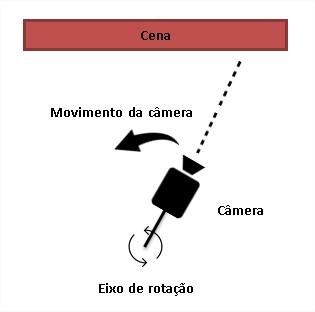
\includegraphics[width=.4\linewidth]{TCC/Imagens/panoramica_padrao.jpg} 
            &
            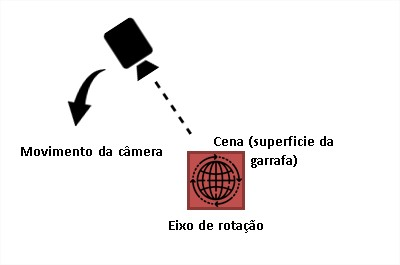
\includegraphics[width=.5\linewidth]{TCC/Imagens/panoramica_trabalho.jpg}
            \\
            (a) Aplicações típicas & (b) Aplicação de inspeção de rótulos.
        \end{tabular}
        \fonte{O autor (2020)}
    \end{minipage}
    \label{fig:gp}
\end{figure}
    
    Existem outras aplicações com essa mesma geometria, cujos autores propõem soluções semi-supervisionadas \cite{lee2000fast} ou propõem soluções de alto custo de hardware (baseadas em \textit{scanners} 3D) e de processamento \cite{Kovacs:2006}, enquanto as linhas de produção de bebidas produzem em velocidades típicas que variam de 2,5 a 15 garrafas por segundo. Além disso, as condições de aquisição em linhas de envase de bebidas são mais facilmente controladas e o produto sob inspeção possui uma geometria substancialmente mais simples que em \cite{lee2000fast,Kovacs:2006}, o que potencialmente possibilita o uso de técnicas igualmente mais simples (e portanto computacionalmente menos custosas) e com resultados mais confiáveis \cite{Park:2013}.
    
    O presente trabalho estuda a aplicação do método proposto em \cite{Lin:2013}, porém sem o uso de algoritmos de registro. Para tanto, o deslocamento entre as cenas é assumido conhecido, com base na posição das quatro câmeras. 
    
    O presente texto está dividido em cinco capítulos. Este primeiro Capítulo é introdutório e, na próxima seção, ainda são apresentados os objetivos do trabalho. O segundo Capítulo descreve a teoria necessária para realizar o mapeamento das distorções, compensações geométricas e a técnica utilizada por \cite{Lin:2013} para a montagem de um mosaico. O método proposto é apresentado no Capítulo 3. No Capítulo 4 são apresentados e discutidos os resultados obtidos. Por fim, o Capítulo 5 finaliza o trabalho.

	\section{Objetivos}
	
	\subsection*{Objetivo geral}
        Gerar uma imagem panorâmica da superfície de um objeto cilíndrico.
	\subsection*{Objetivos específicos} \label{sec:objetivos:especificos}
	\begin{enumerate}
		\item Investigar uma técnica potencialmente adequada à construção de imagens panorâmicas da superfície de garrafas;
		\item Avançar o conhecimento do Núcleo de Inovação e Desenvolvimento em Controle e Automação, da Universidade de Caxias do Sul, a respeito de técnicas de mosaico de imagens;
		\item Avançar o conhecimento do Núcleo de Inovação e Desenvolvimento em Controle e Automação, da Universidade de Caxias do Sul, na direção do desenvolvimento de um inspetor de rótulos para linhas de envase de bebidas.
	\end{enumerate}

\chapter{Fundamentação Teórica}

Para uma série de aplicações, a maneira mais adequada de se obter imagens da superfície de um objeto cilíndrico é adquirir fotografias dessa superfície a partir de diferentes ângulos e, posteriormente, realizar a união destas imagens através de algoritmos de registro utilizados em imagens panorâmicas e outros tipos de mosaicos de imagens \cite{Park:2013}. 
Com a intenção de diminuir deformações causadas pelas distorções projetivas, bem como pelas diferentes perspectivas de projeção geradas pela geometria tridimensional do objeto de interesse, em \cite{Lin:2013} é proposto um algoritmo que corrige essas distorções, utilizando técnicas de trigonometria que proporcionam a identificação de uma coordenada específica da imagem  que representa uma distorção por ângulo. Estes pontos são submetidos a uma transformação geométrica de acordo com a sua posição na imagem.  Neste capítulo, o método proposto em \cite{Lin:2013}, bem como sua aplicação, é detalhado.

\section{Construção das imagens}

A solução proposta em \cite{Lin:2013} se baseia na fusão de imagens obtidas através de ângulos distintos, a fim de ilustrar diferentes regiões da superfície de um cilindro. A Figura~\ref{fig:cameras} representa uma vista superior da disposição entre a garrafa e as quatro câmeras posicionadas com o objetivo de garantir uma visão completa do perímetro do objeto.  

\begin{figure}[ht]
    \caption{Vista superior da disposição das câmeras.}
    \centering
     \vspace{0.4cm}
    \begin{minipage}{.5\textwidth}
        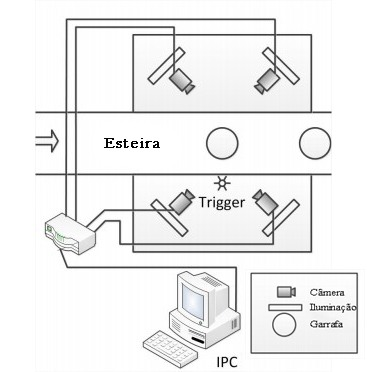
\includegraphics[width=\linewidth]{TCC/Imagens/cameras.jpg}
        \fonte{Adaptado de Lin et al. (2013).}
	\end{minipage}
    \label{fig:cameras}
\end{figure}


Neste sistema, uma esteira realiza o movimento da garrafa que, quando posicionada em frente ao \textit{trigger}, dispara o comando de captura fazendo com que todas as imagens sejam obtidas simultaneamente. Por fim, estas imagens são enviadas ao IPC (\textit{Industrial Personal Computer}) que é responsável por processá-las.

Basicamente, três tipos de distorções são encontradas em imagens adquiridas no contexto deste sistema. O primeiro corresponde às distorções projetivas geradas pelo desalinhamento do plano do sensor com o plano da imagem (cena). O segundo diz respeito às distorções projetivas causadas pela projeção de um objeto (cena) tridimensional em um plano (sensor de aquisição). O terceiro diz respeito às distorções geradas pelo conjunto óptico, principalmente as distorções geométricas geradas pela objetiva. O primeiro tipo de distorção é tratado em \cite{Lin:2013} por meio da  biblioteca de calibração \textit{Camera Calibration Toolbox} do Matlab\textsuperscript{\tiny\textregistered} \cite{CameraCalibration}. Visando a avaliação de uma solução que dispense processos elaborados de calibração, neste trabalho, a compensação desse tipo de distorção é negligenciada. O mapeamento das demais distorções é abordado na seção seguinte.

\subsection{Projeções cilíndricas}

A projeção de um objeto (aproximadamente) cilíndrico no plano do sensor gera distorções nas direções vertical e horizontal. É possível dizer que todas as representações de superfícies curvas em um plano envolvem “contrações” ou “extensões” que podem resultar em distorções ou “rasgos” na tentativa de corrigir estes artefatos através de compensações  geométricas \cite{Shen:2013}. Diferentes técnicas de identificação e representação dessas distorções são utilizadas no sentido de se alcançar resultados que possuam certas propriedades favoráveis para um propósito específico \cite{Shen:2013, Zhao:2013}. 

\begin{figure}[ht]
    \caption{Diagrama esquemático da distorção causada no eixo horizontal.}
    \centering
    \vspace{0.4cm}
    \begin{minipage}{.3\textwidth}
         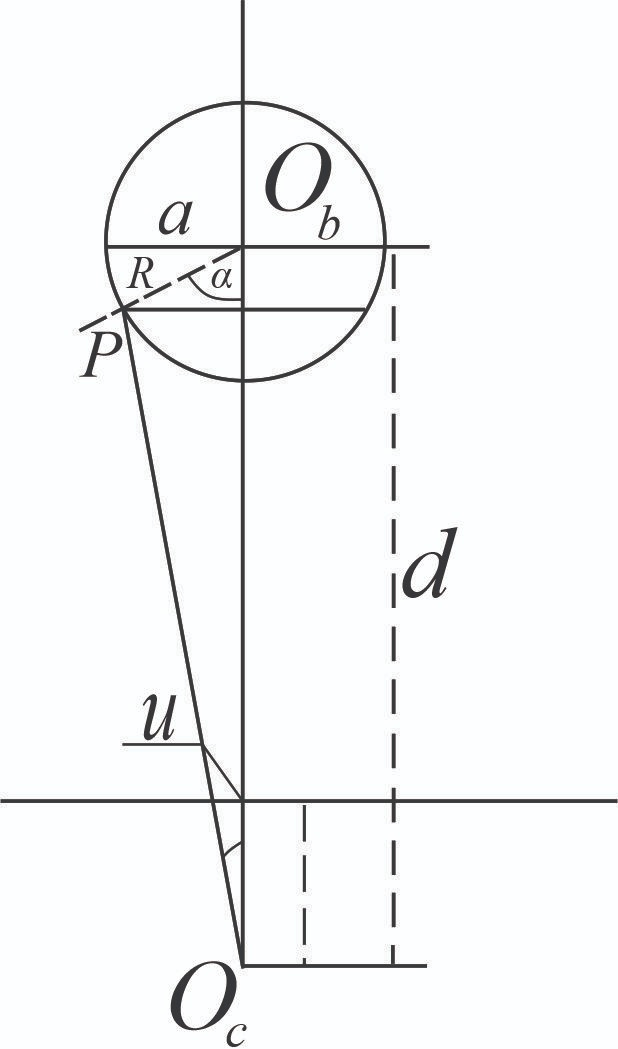
\includegraphics[width=\textwidth]{TCC/Imagens/dist_horz_2.jpeg}
         \fonte{Adaptado de Lin et al. (2013).}
	\end{minipage}
    \label{fig:dist_horz}
\end{figure}


A fim de obter as coordenadas que mapeiam a distorção do eixo $x$ (horizontal), em \cite{Lin:2013} foi considerado o diagrama esquemático apresentado na Figura~\ref{fig:dist_horz}. Nesse diagrama, $u$ representa a coordenada $x$ do ponto $P$ e $\alpha$ denota o ângulo entre os segmentos de reta   $\overline{O_{b}P}$ e $\overline{O_{b}O_{c}}$.  Observando o diagrama é possível estabelecer, através de relações trigonométricas, a função que representa as distorções horizontais, dada por

\begin{equation}
    u = a \frac{\sqrt{d^2 - R^2} \sin{(\alpha)}}{d - R\cos{ \left (\alpha \right)}}
    \label{equacao:dist_horz} 
\end{equation}
em que $R$ é o raio do cilindro (garrafa), $a$ é a distância entre o ponto extremo horizontal (da garrafa) e o seu respectivo centro (na imagem) e $d$ é a distância entre o centro óptico da câmera, $O_{c}$, e o centro da garrafa, $O_{b}$. Levando em consideração que calibrações intrínsecas à câmera estão sendo negligenciadas (não permitindo o real dimensionamento do ângulo máximo real alcançado pelo sensor), neste trabalho o limite lateral esquerdo da garrafa será considerado ideal, representando -90$^\circ$ enquanto o seu ângulo de meia volta identifica o limite à direita do rótulo.

\iffalse
Olha, estive procurando alguns nortes com relação a essa questão da causa desta distorção vertical... Quando se trata de distorção diretamente da lente, acontece o "barrel effect", onde a distorção também deveria ser causada pelos lados..
Alguns sites (não achei nada cientificamente apontado pra isso) demonstram a característica de elipse de acordo com o ponto de visão no objeto cilindrico:
http://kaplanpicturemaker.com/perspective/cylinders (up and around)
https://ariartlessons.wordpress.com/2012/06/12/cylinders-in-perspective/

Aqui os autores do site comentam que esse efeito é causado pela perspectiva, assim como quando desenhamos um cilindro em isometrica, a parte inferior tem o traço de uma elipse na parte inferior. Pelo que eu entendi, caso a foto seja tirada de uma distancia maior, esse efeito pode vir a desaparecer por completo (diminuindo o angulo vertical entre o sensor da câmera e o ponto de maior ordenada da garrafa). Infelizmente eu não sei o que afirmar aqui, na minha interpretação, acaba sendo uma questão de perspectiva.

não sei se poderia referenciar isso sem um embasamento sólido em qualquer um dos casos

\fi
 
Em \cite{Lin:2013} as distorções geradas pela a \iffalse curvatura da lente e pela\fi perspectiva da cena em relação ao eixo vertical são modeladas como uma elipse, assim como é ilustrado na Figura~\ref{fig:dist_vert}, onde a Figura~\ref{fig:dist_vert}~(a) representa o rótulo ideal (sem distorções verticais) e a Figura~\ref{fig:dist_vert}~(b) demonstra o efeito da distorção causado na fotografia. Na imagem em que o rótulo não apresenta distorções, é possível observar que apesar de todos os pontos entre $P_{a}$ e $P_{b}$ terem a mesma ordenada a distorção projetiva causa uma forma geométrica distinta ao plano da imagem obtida, representada no diagrama ao lado. Na figura distorcida, nota-se que quando o ponto se encontra acima do ponto central da imagem, a elipse tem o segmento de curva para cima e quando o ponto se encontra abaixo, tens o segmento inferior da elipse. Na Figura~\ref{fig:dist_vert}~(b) os pontilhados auxiliam na visualização da forma geométrica completa da elipse.


\begin{figure}[ht]
    \caption{Diagrama da distorção vertical. (a) Imagem sem a distorção; (b) Imagem distorcida.}     
    \centering
    \vspace{0.3cm}
    \begin{minipage}{.5\textwidth}
      \centering
            \begin{tabular}{cc}
            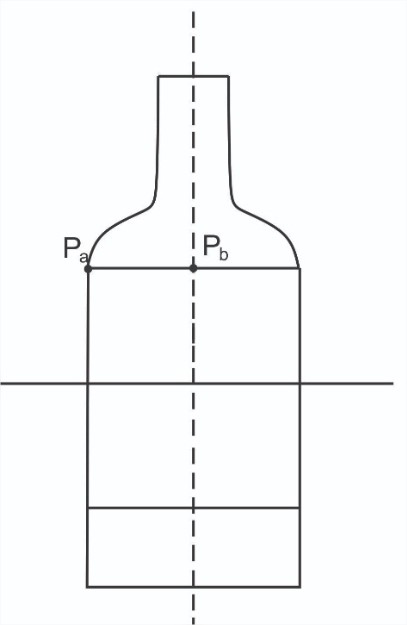
\includegraphics[width=.5\linewidth]{TCC/Imagens/dia_vert_plan.jpg} 
            &
            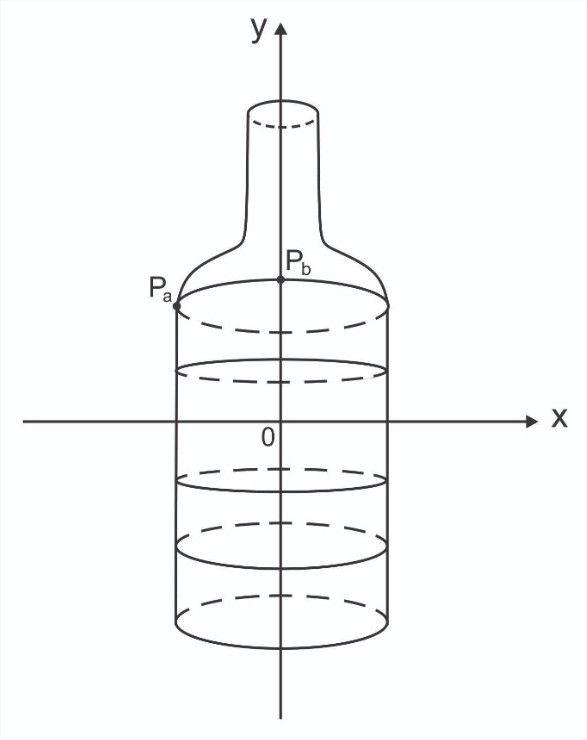
\includegraphics[width=.55\linewidth]{TCC/Imagens/diag_vert_dist.jpg}
            \\
            (a) & (b)
            \end{tabular}
        \fonte{O autor (2020).}
	\end{minipage}
    \label{fig:dist_vert}
\end{figure}

 
Para um melhor entendimento da equação que representa as distorções verticais, se vê necessária uma breve abordagem na equação fundamental que representa a elipse no plano cartesiano (ver Figura~\ref{fig:ellipse_imagem}). Em geometria, uma elipse é um tipo de seção cônica, isto é, caso uma superfície cônica seja cortada por um plano que não passe pela sua base e que não ultrapasse as duas folhas do cone, a interseção entre o cone e o plano é uma elipse. As medidas da elipse são dadas pela metade dos eixos maior e menor sendo chamadas, respectivamente, de semi-eixo maior ($a$) e semi-eixo menor ($b$). A equação fundamental da elipse é dada por

\begin{equation}
    \frac{x^2}{a^2} + \frac{y^2}{b^2} = 1
    \label{equacao:ellipse}
\end{equation}

\begin{figure}[htb]
    \caption{Forma geométrica de uma elipse representada no plano cartesiano.}
    \centering
    \begin{minipage}{.5\textwidth}
      \centering
         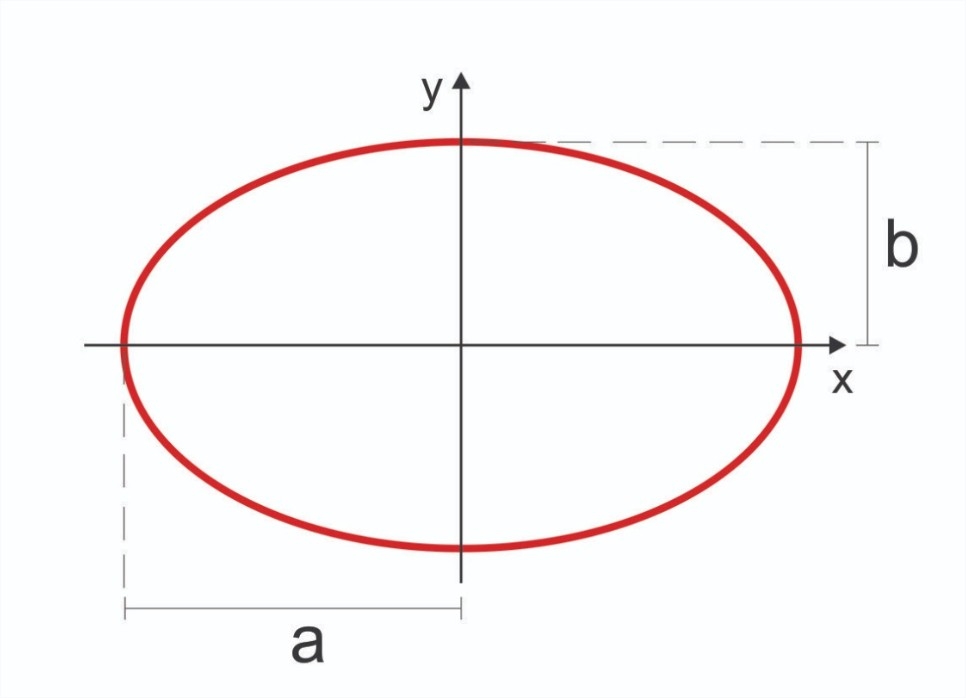
\includegraphics[width=.95\linewidth]{TCC/Imagens/ellipse_imagem.jpg}
         \fonte{O autor (2020).}
	\end{minipage}
    \label{fig:ellipse_imagem}
\end{figure}

Com isso, \citet*{Lin:2013} mapeiam as distorções verticais através da equação descrita a seguir:

\begin{equation}
    %b\sqrt{1 - \frac{u^2}{a^2}} =
    v = h \frac{R}{d+R} \sqrt{1 - \frac{(d^2 - R^2)\sin^2{(\alpha)}}{[d - R\cos{ (\alpha)}]^2}}
    \label{equacao:dist_vert}
\end{equation}
em que $h$ representa a distância entre o centro do rótulo e sua ordenada máxima (na imagem), chamada de $v_{max}$. Uma representação da elipse que identifica uma distorção vertical pode ser vista na Figura~\ref{fig:bottle_ellipse}.


\begin{figure}[htb]
    \caption{Forma geométrica de uma elipse representando a distorção do eixo vertical.}
    \centering
    \vspace{0.3cm}
    \begin{minipage}{.5\textwidth}
      \centering
         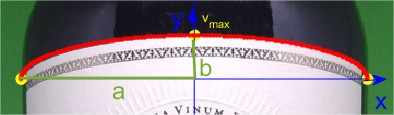
\includegraphics[width=.95\linewidth]{TCC/Imagens/ellipse_apre.jpg}
         \fonte{O autor (2020).}
	\end{minipage}
    \label{fig:bottle_ellipse}
\end{figure}

Com as coordenadas $u$ e $v$ que representam as distorções horizontais e verticais respectivamente identificadas, é possível expandir (realizar as compensações geométricas) a imagem a partir dos pontos mapeados pelo ângulo $\alpha$. Realizando este procedimento com cada uma das imagens, serão formadas no total quatro novas imagens planificadas que, ao se unirem, representarão o perímetro total da garrafa.

\subsection{Compensações geométricas}

Em \cite{Lin:2013} não é detalhado o método adotado para realizar as compensações geométricas. Portanto, nesta revisão são consideradas transformações geométricas a partir do mapeamento das distorções identificadas na imagem. Segundo \cite{Gonzales:2000}, uma transformação geométrica consiste na operação de uma transformação espacial na imagem, sendo essa, responsável pela ''reorganização'' dos pixeis através de regras pré-estabelecidas. Para deixar o procedimento mais claro, será mencionado o exemplo utilizado em \cite{Gonzales:2000}:

Supondo que uma imagem denominada $f$ com coordenadas de pixeis definidas por $(x,y)$ seja submetida a uma transformação geométrica para se tornar uma nova imagem $g$, onde suas novas coordenadas serão dadas por $(x',y')$, a transformação é dada pela seguinte notação:

\begin{equation}
    \begin{array}{l}
        x'= r(x,y) \\
        y'= s(x,y)
    \end{array}
\end{equation}
em que $r(x,y)$ e $s(x,y)$ são as transformações que produzem uma nova imagem $g(x', y')$. Por exemplo, se $r(x,y) = {x}/{2}$ e $s(x,y) = {y}/{2}$, a distorção pode ser descrita como um ``achatamento'' de $f(x, y)$, reduzindo seu tamanho pela metade em ambos os eixos.

O método mais utilizado para modelar essa transformação é a seleção de \textit{tiepoints}, que são coordenadas conhecidas na imagem distorcida e na imagem original \cite{Gonzales:2000}. Na Figura~\ref{fig:spatial_transform_gonzales} é possível visualizar um paralelogramo (figura distorcida) e um quadrado (figura corrigida), onde os \textit{tiepoints} são destacados pelos vértices.

\begin{figure}[htb]
    \caption{Pontos correspondentes em diferentes segmentos de imagem.}
    \centering
    \begin{minipage}{.5\textwidth}
      \centering
         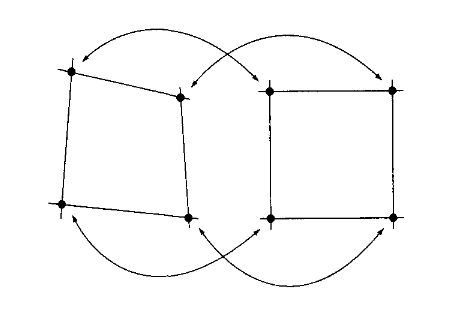
\includegraphics[width=1\linewidth]{TCC/Imagens/spatial_transform.png}
         \fonte{Gonzales e Woods (2000).}
	\end{minipage}
    \label{fig:spatial_transform_gonzales}
\end{figure}


Uma (matriz de) transformação comumente utilizada e que é consistente com o problema abordado neste trabalho é a (matriz de) transformação projetiva. Essa transformação, causa o efeito de inclinação sob o plano da imagem, onde normalmente as linhas paralelas convergem para um ''ponto de fuga'' (ver Figura~\ref{fig:projective_transf}). A equação que descreve uma transformação geométrica na imagem é dada por \cite{Wolberg:1990} como

\begin{equation}
    [x',y',w'] = [u, v, w]  \mathbf{T}
    \label{equacao:matriz_transform}
\end{equation}
em que
\begin{equation}
    \mathbf{T} = 
    \begin{bmatrix}
    a_{11} &  a_{12} & a_{13} \\
    a_{21} &  a_{22} & a_{23} \\
    a_{31} &  a_{32} & a_{33}
    \end{bmatrix}
    \nonumber
\end{equation}
e $[x',y',w']$ é a coordenada homogênea\footnote{Coordenadas homogêneas são um sistema de coordenadas utilizadas em geometria projetiva, assim como coordenadas cartesianas são utilizadas em geometria Euclidiana. A vantagem delas é que pontos, incluindo pontos no infinito, podem ser representados por coordenadas finitas. Formulações que envolvem coordenadas homogêneas são geralmente mais simples e simétricas que as respectivas formulações para coordenadas cartesianas. \cite{August:1997}} de $\mathbf{p} = [x ,y]$.

Diferente de uma transformação afim (mudança de escala, movimento de rotação ou translação), os valores da última coluna são diferentes de zero \cite{Wolberg:1990}. Portando, $a_{13}$ e $a_{23}$ influenciam diretamente no ``ponto de fuga'', de maneira que, quanto maiores são os seus valores, mais o ponto de fuga se aproxima da origem e, portanto, as linhas paralelas parecem convergir mais rapidamente, proporcionando uma inclinação maior no plano da imagem, causando uma ''sensação'' de profundidade na cena (ver Figura~\ref{fig:projective_transf}. Portanto, o mapeamento (fora da forma homogênea) entre a imagem transformada e a imagem original é dado por
 
 \begin{equation}
    \begin{array}{l}
        x = \frac{x'}{w'} = \frac{a_{11}u + a_{21}v+ a_{31}}{a_{13}u + a_{23}v+ a_{33}} \\
        \\
        y = \frac{y'}{w'} = \frac{a_{12}u + a_{22}v+ a_{32}}{a_{13}u + a_{23}v+ a_{33}}
    \end{array}
    \label{equacao:map_transform}
\end{equation}

\begin{figure}[htb]
    \caption{Demonstração de uma transformada geométrica projetiva.}
    \centering
    \begin{minipage}{.9\textwidth}
        \centering
        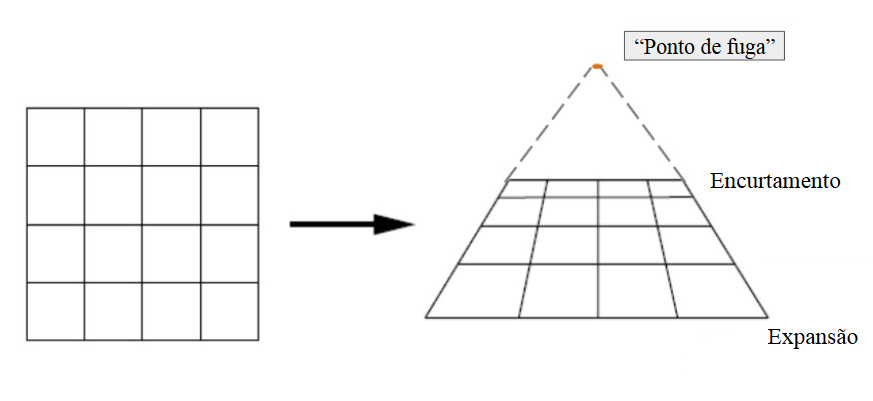
\includegraphics[width=\textwidth]{TCC/Imagens/transform.jpg}
         \fonte{O autor (2020).}
	\end{minipage}
    \label{fig:projective_transf}
\end{figure}


% Em \cite{Wolberg:1990} é afirmado que o mapeamento projetivo inverso é calculado diretamente em termos da matriz inversa de $T$. Portanto, a maneira mais fácil de transformar o plano distorcido em um plano retificado (um paralelogramo para um retângulo, por exemplo) e com a utilização da equação \ref{equacao:inverse_transform}.

% \begin{equation}
%   T^{-1} = \frac{adj(T)}{det(T)}
%     \label{equacao:inverse_transform}
% \end{equation}

% em que $adj(T)$ é a matriz adjunta e $det(T)$ é a sua determinante.\\

Observando que a matriz $\mathbf{T}$ possui dimensões $3\times3$, é possível afirmar que sua normalização resulta em $a_{33}$ = 1, garantindo oito ``termos livres'' na matriz. Com isso, é possível estabelecer uma transformação geométrica projetiva a partir dos quatro pontos conhecidos (\textit{tiepoints}) na imagem original e quatro pontos na imagem distorcida.

Pode-se ressaltar a afirmação de \cite{Gonzales:2000} novamente, em que a utilização de \textit{tiepoints} para modelar a transformação entre ambas as imagens pode ser estabelecida. Em \cite{Wolberg:1990} e \cite{Heckbert:1989} os autores exploram a fundo métodos que aceleram os procedimentos de transformada geométrica, considerando comportamentos conhecidos entre as coordenadas das imagem distorcida e da imagem retificada e melhoria de desempenho, entre outros fatores.

\iffalse
R. Gonzalez, “Digital Image Processing,” Section 5 11 Section 5.11
George Wolberg, Digital Image Warping, Wiley-IEEE Computer Society Press, 1990
\fi

\subsection{Mosaico de imagens}

A construção de uma imagem panorâmica é uma técnica que reúne múltiplas imagens adquiridas a partir de diferentes vistas. O principal objetivo é formar uma imagem única e abrangente, também chamada de mosaico \cite{Shum:2000}. Para que o mosaico tenha uma qualidade considerável, a união das imagens (também conhecida por ``fusão'') é um dos passos mais importantes. Esse tipo de técnica se baseia em premissas matemáticas que demandam, por exemplo, a existência de semelhanças e sobreposições consideráveis entre regiões das diferentes imagens a serem fundidas. Entretanto, é comum que ocorram variações geométricas nas áreas de sobreposição das imagens ou violações nessas premissas durante o processo de aquisição, acarretando em artefatos degradantes, como regiões desfocadas ou costuras visíveis entre as imagens \cite{Gracias:2009}.

Em \cite{Levin:2004}, as técnicas de mosaico são divididas em duas abordagens: suavizações entre transições; e localizações ideais de costura. O trabalho proposto em  \cite{Lin:2013} segue a segunda abordagem, visando obter um resultado mais preciso na união das imagens. Dessa forma, foi empregada uma técnica de registro de imagens que permite contornar os problemas de mudança de escala, variações de iluminação e 
a possibilidade da garrafa ser apresentada para as câmeras rotacionada (em diferentes posições angulares). Dentre as diversas técnicas disponíveis para a detecção de características comuns entre imagens em \cite{Lin:2013} foi utilizado o método SIFT (\textit{Scale-invariant feature transform}), este, pode ser considerado como uma espécie de detector de bordas/linhas que apresentam características padrões na imagem  \cite{Lowe:2001}. Segundo \cite{Mikolajczyk:2005}, o algoritmo SIFT é um dos métodos que obtêm os melhores resultados de correspondência entre pontos, levando em consideração os problemas mencionados.

Em cada uma das imagens, já com as distorções compensadas, o algoritmo é utilizado a fim de identificar \textit{key points} (também chamados de \textit{pontos descritores}, em português), estes pontos são responsáveis pela identificação das bordas mais relevantes da imagem (normalmente baseados em uma frequência). Na Figura~\ref{fig:SIFT} é possível visualizar uma imagem com seus \textit{key points} destacados em vermelho. 

Em pares, as imagens são submetidas a um processo de comparação entre seus respectivos \textit{key points}, identificando características em comum entre os pontos descritores de ambas. Os pontos descritores que tem a maior taxa de similaridade entre si (pixels vizinhos que apresentam o mesmo padrão, por exemplo) são considerados o mesmo ponto no espaço, ou seja, o ponto ideal de costura entre as imagens. Para a realização dessa tarefa, é necessário gerar uma matriz de homografia.

\begin{figure}[htb]
    \caption{Destaque dos \textit{key points} da imagem, obtidos com a utilização do SIFT.}
    \label{fig:SIFT}
    \centering
	\vspace{0.4cm}
	\begin{minipage}{.7\textwidth}
	    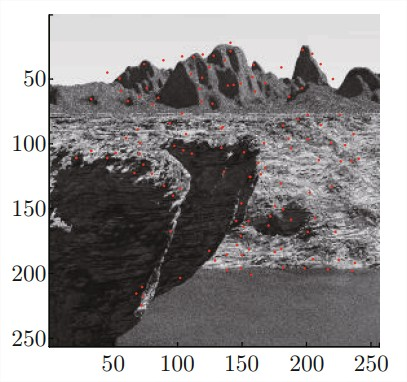
\includegraphics[width=\textwidth]{TCC/Imagens/SIFT.jpg}
	    \fonte{Wang et al. (2017).}
	\end{minipage}
\end{figure}

Em \cite{Gledhill:2003} uma matriz de homografia é definida como um mapeamento entre duas imagens de uma superfície planar, constituindo uma única cena, adquiridas de perspectivas diferentes. Ou seja, duas imagens de uma mesma cena estão relacionadas por uma matriz de homografia (normalmente de dimensão $3\times3$, representando escala, rotação e translação entre as imagens). Essa matriz pode ser utilizada para remapear as imagens a partir de diferentes planos. Na Figura~\ref{fig:RANSAC_OUTLIER} é possível observar o resultado da correspondência de características (obtidas através do SIFT) entre imagens da mesma cena, obtidas de planos distintos.

\begin{figure}[htb]
    \caption{Exemplo de correspondência entre pontos com a utilização do SIFT. }
    \centering
    \vspace{0.3cm}
    \begin{minipage}{.9\textwidth}
         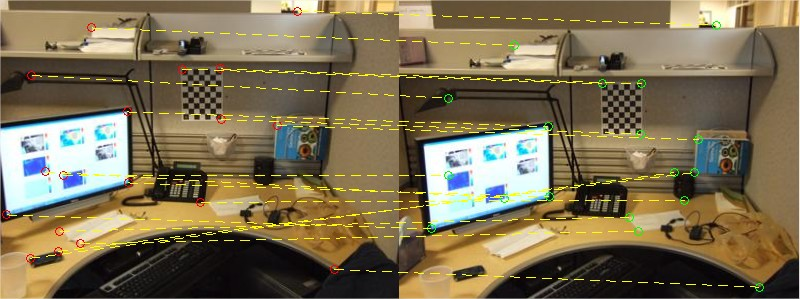
\includegraphics[width=\textwidth]{TCC/Imagens/RANSAC_OUTLIERS.jpg}
         \fonte{\cite{RANSAC}.}
	\end{minipage}
    \label{fig:RANSAC_OUTLIER}
\end{figure}

A fim de evitar problemas de registro, é necessário verificar se pontos de correspondência não foram estimados incorretamente. Para isso, é utilizado o algoritmo RANSAC (\textit{Random Sample Consensus}), que é um método iterativo para estimar um modelo matemático de um conjunto de dados que contém pontos que fogem do
padrão estatístico, chamados de \textit{outliers}, e pontos que estão dentro deste padrão, denominados \textit{inliers} \cite{Fischler:1981}. Com a classificação desses dados
concluída, é possível gerar uma nova matriz de homografia considerando apenas as coordenadas em ambas as imagens que estejam dentro do modelo matemático gerado. A remoção 
dos \textit{outliers} é demonstrada na Figura~\ref{fig:RANSAC_INLIERS}, melhorando consideravelmente a taxa de acerto na correspondência entre pontos nas duas imagens.

\begin{figure}[htb]
    \caption{Remoção dos \textit{outliers} com a utilização do RANSAC. }
    \centering
    \vspace{0.3cm}
    \begin{minipage}{.9\textwidth}
         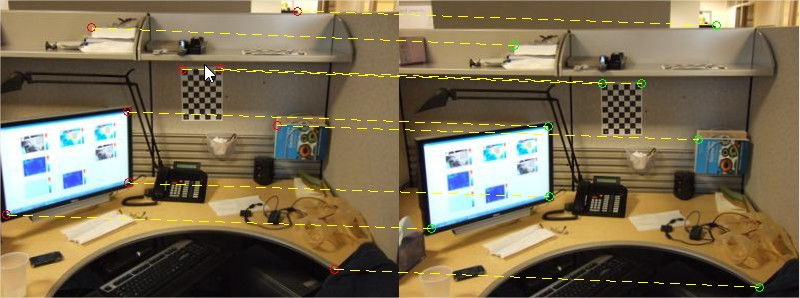
\includegraphics[width=\textwidth]{TCC/Imagens/RANSAC_INLIERS.jpg}
         \fonte{\cite{RANSAC}.}
	\end{minipage}
    \label{fig:RANSAC_INLIERS}
\end{figure}


Finalmente, com a melhor matriz de homografia definida, agora é possível realizar a fusão deste par de imagens. Em \cite{Lin:2013}, os autores não mencionam o método que utilizaram 
para realizar a fusão das imagens, todavia é necessário utilizar algum método para corrigir artefatos que são causados pela sobreposição das imagens unidas. Realizando a união de todas as imagens, é possível visualizar todo o perímetro da garrafa com uma única imagem.



\chapter{Método proposto} 

Este capítulo trata da estratégia utilizada para a aquisição das imagens que será utilizada na implementação do algoritmo. Além disso, é definido o escopo e são apresentados detalhes da implementação do método proposto em \cite{Lin:2013}, que serve de base para o mapeamento das distorções avaliadas neste trabalho. Os métodos adotados para a compensação das distorções e montagem do mosaico também  são descritos a seguir.

\section{Plataforma de aquisição}
O experimento será realizado basicamente com três elementos: um objeto cilíndrico de referência (garrafa); uma câmera digital para obtenção das imagens em torno do eixo do objeto cilíndrico; e, por fim, uma plataforma que auxilia no movimento rotacional da garrafa.

O objeto de interesse trata-se de uma garrafa, de vinho, com rótulo frontal e traseiro. Ainda que a produção de vinhos seja substancialmente menor que a produção de cerveja, uma garrafa típica de cerveja tem um formato mais próximo de um cilindro que a garrafa considerada, o que leva a menores distorções e, portanto, a um desempenho melhor dos algoritmos.     

O dispositivo de aquisição utilizado é a câmera traseira de um \textit{smartphone} ASUS, modelo Zenfone 3, com resolução de $4656 \times 2620$ píxeis. A câmera é posicionada para aquisições em formato retrato (\textit{portrait}) a uma distância adequada ao enquadramento integral da garrafa no campo de visão, adicionadas pequenas margens de segurança. 

A garrafa e o sistema de aquisição são colocados em frente a um fundo verde, de forma a gerar uma imagem de alto contraste e de facilitar a segmentação, que não está propriamente no escopo deste trabalho. A câmera (única) é mantida fixa, enquanto a garrafa é rotacionada em passos de $90^\circ$. Com isso, são simuladas aquisições de imagens de uma garrafa fixa a partir de diferentes câmeras.

A rotação da garrafa é implementada com o auxílio de uma plataforma giratória. Essa plataforma possui um formato quadrado com a intenção de facilitar a rotação controlada de $90^\circ$, podendo ser dividida em duas partes, sendo a parte inferior responsável pela fixação e preservação do local em que a plataforma se encontra e a parte superior encarregada de realizar o movimento de rotação da garrafa. Os lados de ambas partes (superior e inferior) sempre permanecem alinhados, garantindo a movimentação correta entre a aquisição das imagens. Na plataforma superior são inseridos marcadores angulares, simulando a posição (angular) das câmeras dispostas em torno do eixo da garrafa. A Figura~\ref{fig:plat_esq} apresenta um esquemático da plataforma utilizada.

\begin{figure}[htb]
    \caption{Diagrama esquemático da plataforma utilizada para a aquisição das imagens. }
    \centering
    \vspace{0.3cm}
    \begin{minipage}{.5\textwidth}
         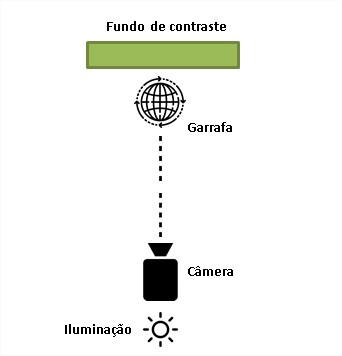
\includegraphics[width=\textwidth]{TCC/Imagens/Esquematico_plataforma.jpg}
         \fonte{O autor (2020).}
	\end{minipage}
    \label{fig:plat_esq}
\end{figure}

\section{Sistema proposto}

Inicialmente, a imagem é submetida a um processo de redimensionamento e seleção da região de interesse. Após esse procedimento, é possível realizar a identificação das distorções de acordo com a quantidade de pontos escolhida pelo usuário. Realizando as compensações geométricas entre os pontos gerados pelo algoritmo, a união das quatro imagens é efetuada, possibilitando uma visão em torno de todo o eixo da garrafa. Um diagrama do sistema proposto é demonstrado na Figura~\ref{fig:diagrama_alg}.

\begin{figure}[htb]
    \caption{Etapas do sistema proposto.}
    \centering
    \vspace{0.3cm}
    \begin{minipage}{\textwidth}
         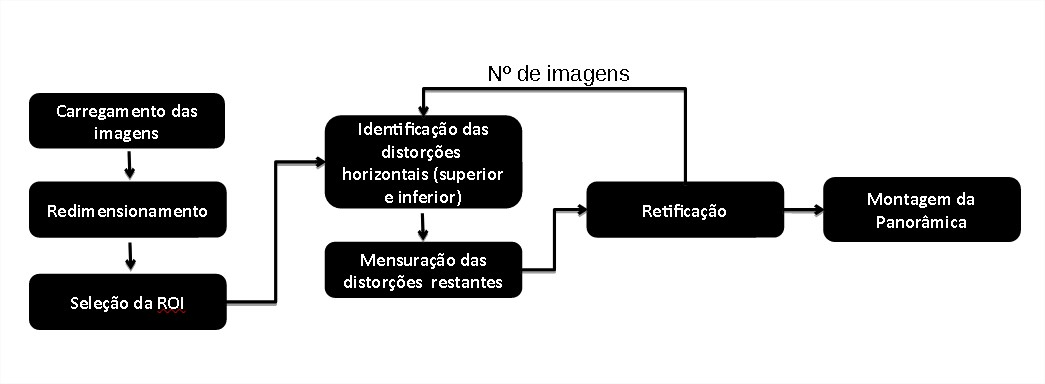
\includegraphics[width=\textwidth]{TCC/Imagens/diagrama_alg.jpg}
         \fonte{O autor (2020).}
	\end{minipage}
    \label{fig:diagrama_alg}
\end{figure}

\section{Pré-processamento da imagem}

As imagens, originalmente com $4656 \times 2620$, são redimensionadas para padrões  HD ($1280 \times 720$). Esse redimensionamento é feito por meio de interpolação bicúbica. São considerados dois tamanhos de imagens para possibilitar uma avaliação da perda de desempenho do método frente à redução da resolução. A redução de dimensão das imagens se dá em função do custo de implementação (o valor de câmera industriais de resolução superior a HD tende a subir significativamente \cite{Webb:2003, Shereena:2015}). Outra razão é a redução no custo computacional, o que, de forma semelhante, impacta nos custos de implementação de um sistema desse tipo.

Seis pontos de interesse, caracterizados pelos limites extremos do maior rótulo (quando observado frontalmente pela câmera) são definidos (por ora, de forma supervisionada). Os pontos que delimitam a região de interesse do algoritmo visam o dimensionamento da elipse causada pela distorção projetiva vertical e são caracterizados pelos seguintes limites (ver Figura~\ref{fig:elipse}):

\begin{enumerate}[label=\arabic*)]
	\item Ponto superior esquerdo;
	\item Ponto de maior ordenada;
	\item Ponto superior direito;
	\item Ponto inferior esquerdo;
	\item Ponto de menor ordenada;
	\item Ponto inferior direito.
\end{enumerate}

Com as coordenadas desses pontos definidas, é possível observar a curva caracterizada geometricamente com o formato de um segmento de elipse, confirmando a representação da distorção afirmada por \cite{Lin:2013}. Na Figura~\ref{fig:elipse} é representado um exemplo da seleção de pontos em uma garrafa em conjunto de uma ilustração da elipse obtida.


\begin{figure}[htb]
    \caption{Pontos que representam as extremidades do rótulo (em amarelo) e a elipse imaginaria (em vermelho).}
    \centering
    \vspace{0.3cm}
    \begin{minipage}{0.4\textwidth}
      \centering
         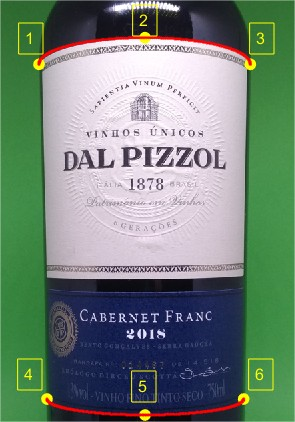
\includegraphics[width=\textwidth]{TCC/Imagens/ellipse.jpg}
         \fonte{O autor (2020).}
	\end{minipage}
    \label{fig:elipse}
\end{figure}

\section{Mapeamento das distorções}

% \cred{<\textit{a pergunta que fica para mim é, precisamos fazer isto?? Não te preocupa com a minha pergunta (depois conversamos sobre isso --- é só para eu me lembrar)}>} 
Para a identificação das distorções projetivas horizontais  e verticais é necessário atribuir a quantidade de pontos horizontais  que  irão representar  o  ``passo'' de ângulo  no  plano  da  imagem.   Uma  quantidade de pontos  maior  proporciona  um  detalhamento  mais  fiel à imagem  planificada,  todavia  isso interfere significativamente no desempenho do algoritmo, demandando um custo computacional mais elevado.
Visto que o mapeamento das distorções é dado pelas equações \eqref{equacao:dist_horz} e \eqref{equacao:dist_vert}, o algoritmo utilizado para a obtenção destas coordenadas é visto no pseudo-código descrito no Algoritmo~\ref{alg:1}.

\begin{algorithm}
    \caption{Mapeamento da Elipse}
    \label{alg:1}
    \begin{algorithmic}[1]
    \Function{map\textunderscore ellipse}{}
    \State $i \gets 1$
    \For{\texttt{$\alpha \gets -\pi/2$ até $\pi/2$ incremente de $\pi/HP$}} \Comment{HP = Pontos horizontais}
        \State $u \gets$ Equação \ref{equacao:dist_horz}
        \If {elipse inferior}
            \State $v \gets$ Equação \ref{equacao:dist_vert} 
        \Else
            \State $v \gets$ $-$ Equação \ref{equacao:dist_vert}
        \EndIf
    \State $Resultado(i) \gets [u, v]$
    \State $i \gets i + 1$
    \EndFor
    \State \Return  $Resultado$
    \EndFunction
    \end{algorithmic}
\end{algorithm}

A variação de $\alpha$ permite obter as coordenadas que representam ambas as distorções.  O que se pode perceber é uma forma geométrica de uma elipse (distorção vertical) com pontos horizontais menos afastados entre si conforme aproximam-se das bordas (limites do rótulo) (distorção horizontal).

Assumindo o diagrama \ref{fig:dist_vert}, nota-se que a caracterização da distorção do eixo vertical vai causando uma perda da excentricidade da elipse conforme se aproxima do centro da figura. Com essa informação é possível concluir que novas elipses devem ser identificadas na área que se delimita aos pontos extremos já conhecidos. 

Para realizar a identificação dos pontos internos (entre as duas elipses estabelecidas supervisionadamente), é possível estabelecer a relação entre as coordenadas das distorções já conhecidas através do pseudo-código transcrito no Algoritmo~\ref{alg:2}, $CES$ e $CEI$ correspondem à coordenada do mesmo ângulo na elipse superior e na elipse inferior, respectivamente.

Basicamente a operação que o algoritmo realiza é a definição de um ''passo'' (que depende da quantidade de pontos verticais), responsável por diminuir a excentricidade da elipse superior. A elipse superior é escrita repetitivamente com a inclinação cada vez menor, até chegar próximo do centro (onde sua inclinação chega muito próxima de zero).

\begin{algorithm}[htb]
    \caption{Mapeamento das demais distorções}
    \label{alg:2}
    \begin{algorithmic}[1]
    \Function{distortion\textunderscore points}{}
     \For{\texttt{$indiceLinha \gets 1$ até $indiceLinha \gets VP$ }} \Comment{VP = Pontos verticais}
         \For{\texttt{$indiceColuna \gets 1$ até $indiceColuna \gets HP$ }} \\
            \State $delta \gets \frac{CES[indiceColuna] - CEI[indiceColuna]}{VP}$ \\
             \State $row[indiceColuna] \gets CES[indiceColuna] - delta * VP$
         \EndFor
        \State $map[indiceLinha] \gets row$
    \EndFor
    \State \Return  $map$
    \EndFunction
    \end{algorithmic}
\end{algorithm}

\section{Compensações das distorções}

Com todos os pontos que representam as distorções existentes no plano da imagem identificados, se vê necessário realizar compensações geométricas a partir deste mapeamento. Para a realização desta tarefa, os valores são armazenados em vetores que representam coordenadas de todos os pontos horizontais a cada índice vertical. A partir deste vetor de armazenamento, sequencialmente, as coordenadas que representam um paralelogramo na imagem, são submetidas a uma transformação geométrica projetiva que irá alterar a forma geométrica (do então paralelogramo), para um bloco com formato retangular com tamanho pré-definido (ver Figura~\ref{fig:quad}).

\begin{figure}[htb]
    \caption{Aplicação da transformada geométrica projetiva no mapeamento das distorções.}
    \centering
    \vspace{0.25cm}
    \begin{minipage}{\textwidth}
      \centering
         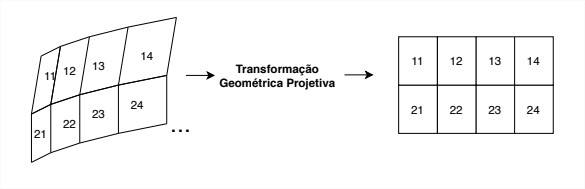
\includegraphics[width=\textwidth]{TCC/Imagens/transform_esq.jpg}
         \fonte{O autor (2020).}
	\end{minipage}
    \label{fig:quad}
\end{figure}


Visando uma representação fiel do rótulo analisado, o dimensionamento da imagem planificada é descrito a seguir. O dimensionado vertical da imagem (planificada) pode ser estabelecido através da distância entre pontos de maior e menor ordenada (definidos pelos pontos atribuídos supervisionadamente). Já o comprimento (total) $C$ da imagem é dimensionado através do tamanho da circunferência que é visualizada na imagem. Utilizando a relação do perímetro da garrafa, é possível definir a largura total da imagem como sendo

\begin{equation}
    C = \frac{2 \pi r}{2} = \pi r
    \label{equacao:largura_imagem}
\end{equation}
em que r, representa o raio da garrafa (em pixels).

Considerando que a imagem total é composta por blocos, cada um deles correspondendo a um ângulo $\alpha$ no plano da imagem original, o dimensionamento horizontal $C$ é dividido igualmente de acordo com a quantidade de pontos horizontais atribuídos. O diagrama da Figura~\ref{fig:esq_bloco} demonstra a lógica que estabelece a compensação geométrica entre os blocos.

\begin{figure}[htb]
    \caption{Esquemático do dimensionamento dos blocos que compõem a imagem.}
    \centering
    \vspace{0.3cm}
    \begin{minipage}{.6\textwidth}
         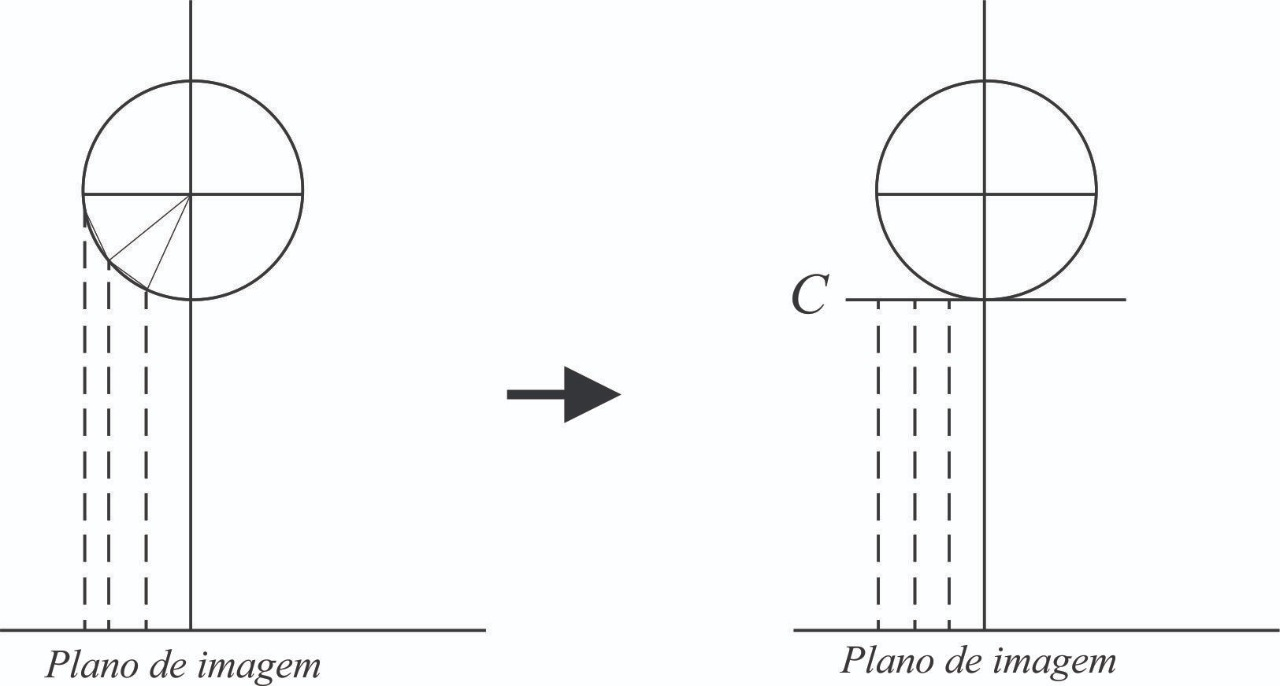
\includegraphics[width=\textwidth]{TCC/Imagens/esq_bloco.jpeg}
         \fonte{O autor (2020).}
	\end{minipage}
    \label{fig:esq_bloco}
\end{figure}

Realizando esse método de compensação com todos os respectivos pontos horizontais e verticais, a imagem planificada é finalmente concluída. Esse procedimento deve ser executado com as demais imagens que representam o deslocamento angular da garrafa, para assim, ser realizada a montagem do mosaico.

\section{Montagem do mosaico}

Diferente do método proposto em \cite{Lin:2013}, que utiliza os algoritmos de registro mencionados no capítulo anterior, neste trabalho optou-se por %utilizar
assumir o movimento da garrafa como conhecido (ou seja, assume-se que a posição das câmeras é conhecida), para realizar a montagem da panorâmica. Os dois principais motivos que justificam a não utilização de algoritmos específicos para o registro de imagens são discutidos a seguir.

Em primeiro lugar, na abordagem de \cite{Lin:2013}, o sistema é empregado para realizar a inspeção em garrafas PET (Polietileno Tereftalato), enquanto neste trabalho avalia-se a inspeção de garrafas que não possuam rótulo que cubra todo o perímetro da garrafa (diferente das garrafas PET, que em sua maioria, apresentam essa característica). Esse detalhe pode vir a impactar diretamente no registro das imagens, visando que as garrafas utilizadas neste trabalho são definidas por grandes áreas de cor homogênea, e a ausência de ``bordas'' e ``cantos'' pode vir a dificultar a detecção de \textit{keypoints} na imagem. Por exemplo, se uma garrafa de vinho não apresentar um rótulo grande o suficiente para compartilhar áreas em comum entre as imagens, o registro pode não conseguir gerar \textit{inliers} o suficiente para calcular uma matriz de homografia responsável por fazer o alinhamento correto das imagens.

O segundo fator aborda o custo computacional exigido pelo algoritmo de registro proposto pelo autor. O método SIFT é constantemente abordado na comunidade científica a fim de propor melhorias de desempenho ao algoritmo, que, apesar de apresentar bons resultados demanda um poder de processamento elevado para detectar os \textit{keypoints} nas imagens \cite{Suzuki:2012}. Somado a isso, na aplicação descrita nesse trabalho deve-se levar em conta o processamento da comparação entre as imagens (minimamente quatro), bem como a transformação e fusão, dificultando a aplicação do método em meio a sistemas de tempo real.

Considerando os problemas descritos, %neste trabalho 
optou-se por assumir que os movimentos relativos entre as imagens são conhecidos. 
A caracterização do movimento conhecido estabelece que o algoritmo já conhece previamente a ordem de arranjo entre as cenas para a montagem do mosaico, bem como a representação angular de cada imagem na panorâmica.

Como já mencionado, o fato deste trabalho estar negligenciando calibrações intrínsecas à câmera e, por isso, cada uma das imagens  planificadas é dimensionada para representar o valor ideal de meio perímetro da garrafa (180$^\circ$), deve ser escolhida a porcentagem de visualização de cada uma das imagens para que cada segmento do mosaico não apresente blocos de imagens repetidos ou faltantes. Assumindo que serão obtidas quatro fotografias em torno do eixo da garrafa, sendo que cada uma dessas representará $90^{\circ}$ de todo o seu perímetro $C$ (idealmente), optou-se pelo descarte de $45^{\circ}$ em cada lado da representação planificada da imagem, assim, a soma da representação angular (na panorâmica) em cada uma das imagens, totalizará o perímetro completo da garrafa.



\chapter{Resultados} 

Este capítulo se destina à apresentação dos resultados obtidos diante da implementação do algoritmo. Na primeira seção, há uma breve descrição da plataforma utilizada para adquirir as imagens. Na segunda seção são demonstrados os resultados obtidos no mapeamento das distorções com a variação de alguns parâmetros fixos. Já na terceira seção, é possível analisar os resultados de imagens já retificadas e, por fim, a quarta seção demonstra o resultado do mosaico obtido após os processamentos realizados na imagem.

\section{Plataforma de aquisição}

As aquisições das imagens foram realizadas em uma plataforma dedicada a fim de obter a maior controle das condições de aquisição. A câmera utilizada teve seus parâmetros automáticos desativados e a exposição foi configurada manualmente, a fim de evitar variações de iluminação entre as diferentes imagens. A câmera fixada um tripé e teve sua inclinação 
ajustada com auxilio de uma ferramenta de nível. Na Figura~\ref{fig:plataforma} é possível visualizar o ambiente onde foram realizados os ensaios.

\begin{figure}[htb]
    \caption{Plataforma utilizada para a aquisição das imagens. }
    \centering
    \vspace{.3cm}
    \begin{minipage}{.4\textwidth}
            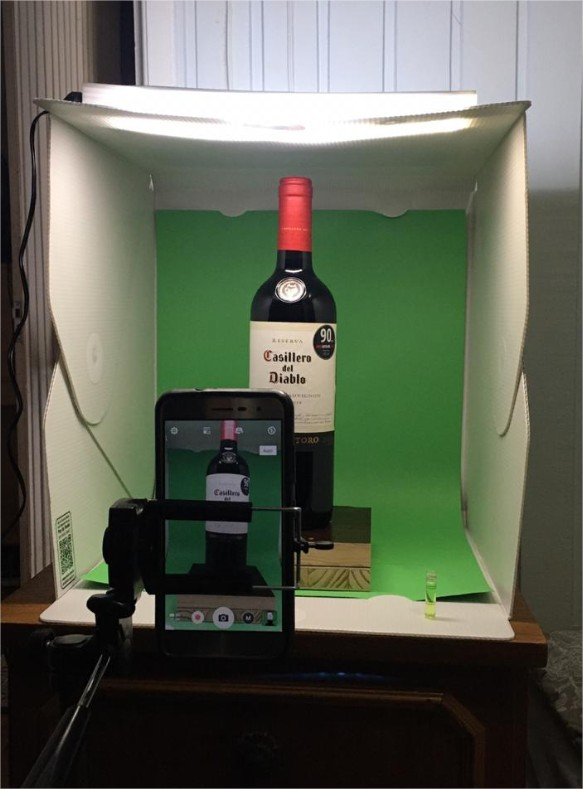
\includegraphics[width=\textwidth]{TCC/Imagens/plataforma.jpg}
            \fonte{O autor (2020).}
	\end{minipage}
    \label{fig:plataforma}
\end{figure}

\section{Identificação das distorções projetivas}

Com a identificação supervisionada dos seis pontos que representam os limites do rótulo efetuada, é necessário fazer o mapeamento das distorções a partir dessas delimitações. As distorções foram identificadas a partir do Algoritmo 1 (Mapeamento da Elipse) com uma escolha de trinta pontos horizontais, facilitando a visualização da caracterização geométrica do método. Na primeira execução, os parâmetros fixos do sistema foram dados por $R = 3,\!5$  e $d= 33$  (ambos em cm). Na Figura~\ref{fig:pontos_horizontal} é possível observar os resultados diante desta reprodução, onde os pontos em vermelho descrevem o mapeamento das distorções e os pontos em amarelo, as coordenadas que delimitam o rótulo.

\begin{figure}[htb]
    \caption{Aplicação do algoritmo para obtenção da distorção. }
    \centering
    \vspace{.3cm}
    \begin{minipage}{.3\textwidth}
      \centering
         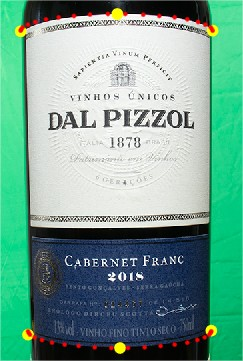
\includegraphics[width=\textwidth]{TCC/Imagens/pontos_horizontal.jpg}
            \fonte{O autor (2020).}
	\end{minipage}
    \label{fig:pontos_horizontal}
\end{figure}
    
O que se pode observar é que os pontos ficaram mais próximos entre si à medida que foram se aproximando do limite do rótulo (representando a distorção horizontal) e também atingiram um padrão geométrico esperado (elipse). As coordenadas restantes foram obtidas através do método descrito no capitulo anterior. Utilizando como parâmetro a presença de trinta pontos horizontais e vinte pontos verticais, a Figura~\ref{fig:total_distor} representa as distorções características a este rótulo perante o plano da imagem.

\begin{figure}[htb]
    \caption{Pontos que representam as distorções características desta garrafa.}
    \centering
    \vspace{.3cm}
    \begin{minipage}{.3\textwidth}
      \centering
         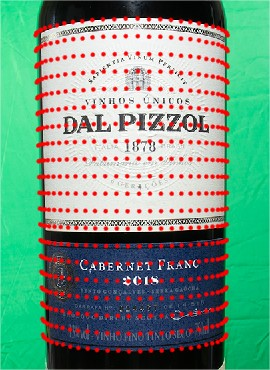
\includegraphics[width=\textwidth]{TCC/Imagens/total_distor.jpg}
            \fonte{O autor (2020).}
	\end{minipage}
    \label{fig:total_distor}
\end{figure}

Nota-se que as distorções mapeadas apresentaram uma característica muito fiel ao diagrama esquemático da Figura~\ref{fig:dist_vert}, onde as elipses de maior ordenada apresentam uma inclinação superior às elipses que se concentram mais próximas do centro do rótulo. Também é possível destacar que o sistema de mapeamento proposto em \cite{Lin:2013} considera que o eixo focal da câmera se encontra minuciosamente alinhado com o centro do rótulo. A alteração de parâmetros fixos ($R$ e $d$) influencia diretamente nos quesitos excentricidade das elipses extremas e, em consequência disso, das elipses internas.

\section{Remoção das distorções}

Para a validação desta etapa, a proposta de ensaio foi a utilização de uma garrafa envolvida por uma folha da papel quadriculado a fim de avaliar visualmente a retificação da imagem. Os desfechos a seguir demonstram o resultado da imagem planificada com diferentes quantidades de pontos verticais e pontos horizontais atribuídos. Na Figura~\ref{fig:ensaio_1a} é possível observar uma fotografia do objeto utilizado para a avaliação de resultados. Todas as execuções foram realizadas com valores ($N$) de pontos horizontais e verticais idênticos, proporcionando uma proporção de pontos de $N \times N$. 

\begin{figure}[ht]
    \caption{Imagem do objeto analisado.}
    \centering
    \vspace{.3cm}
    \begin{minipage}{.2\textwidth}
        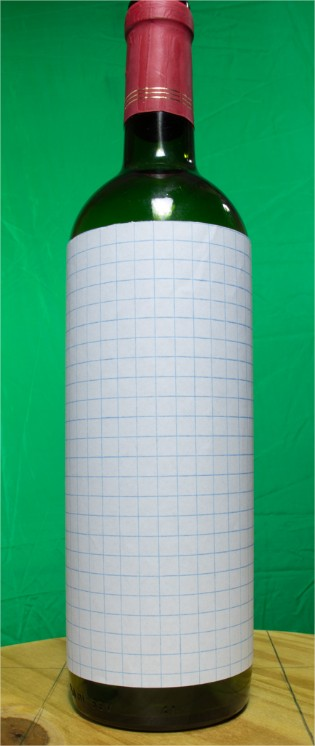
\includegraphics[width=\textwidth]{TCC/Imagens/ensaios/quadriculado.jpg}
        \fonte{O autor (2020).}
	\end{minipage}
    \label{fig:ensaio_1a}
\end{figure}

% \cred{<\textit{aqui ficou estranho... podes colocar resultados em anexo, mas não podes discutir os resultado aqui e colocar as imagens lá... acho melhor trazeres tudo para cá...}>}
A Figura~\ref{fig:ensaio_2_55a} demonstra o primeiro experimento, no qual
foi utilizado um valor de $N = 5$. A imagem à esquerda (a) representa a identificação das $N$ distorções encontradas em cada eixo, enquanto a imagem à direita (b) representa o resultado da imagem planificada. Entre a Figura~\ref{fig:ensaio_2_1010a} e a Figura~\ref{fig:ensaio_2_3030a}, os valores $N$ são dados por 10, 20 e 30, respectivamente, e apresentam a mesma estrutura de apresentação. O que se pode perceber nestes resultados é a melhoria significativa da representação planificada da imagem conforme o valor de $N$ é incrementado. No primeiro resultado, as falhas e distorções são facilmente visíveis conforme se aproximam do limite lateral da imagem. Contudo, os tamanhos dos retângulos são uniformes dentre a área mais central da imagem planificada. 

\begin{figure}[ht]
    \caption{Resultado da planificação com N = 5.}     
    \centering
    \vspace{0.3cm}
    \begin{minipage}{.5\textwidth}
      \centering
            \begin{tabular}{cc}
            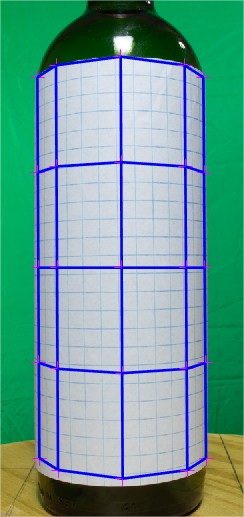
\includegraphics[width=.4\linewidth]{TCC/Imagens/ensaios/a_55.jpg} 
            &
            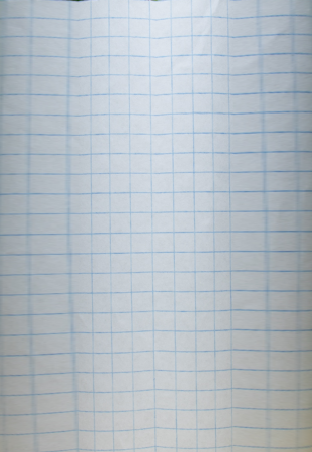
\includegraphics[width=.55\linewidth]{TCC/Imagens/ensaios/b_55.png}
            \\
            (a) Imagem original & (b) Imagem planificada.
            \end{tabular}
        \fonte{O autor (2020).}
	\end{minipage}
    \label{fig:ensaio_2_55a}
\end{figure}

\begin{figure}[ht]
    \caption{Resultado da planificação com N = 10.}     
    \centering
    \vspace{0.3cm}
    \begin{minipage}{.5\textwidth}
      \centering
            \begin{tabular}{cc}
            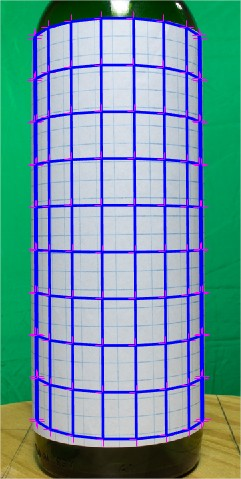
\includegraphics[width=.4\linewidth]{TCC/Imagens/ensaios/a_1010.jpg} 
            &
            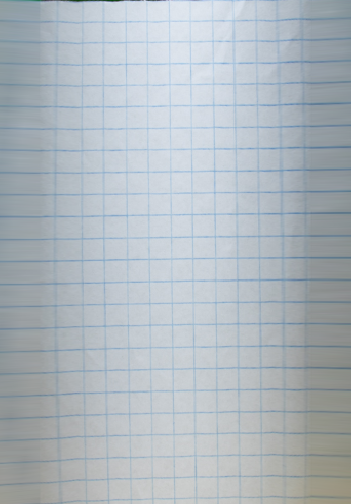
\includegraphics[width=.55\linewidth]{TCC/Imagens/ensaios/b_1010.png}
            \\
            (a) Imagem original & (b) Imagem planificada.
            \end{tabular}
        \fonte{O autor (2020).}
	\end{minipage}
    \label{fig:ensaio_2_1010a}
\end{figure}

No segundo experimento, apesar de uma melhor atribuição ao tamanho dos retângulos, ainda é possível destacar a presença de borrões. Além disso, o último retângulo de cada lado não apresenta uma última linha vertical, formando um retângulo maior. Por fim, os últimos dois experimentos se demonstraram sem a presença de deformações aparentes dentre as imagens resultantes. Todavia, é importante observar que com $N = 30$, apesar de pouco perceptível, a imagem apresenta a última linha vertical levemente mais visível e uniforme, se comparada ao caso em que $N = 20$.

\begin{figure}[ht]
    \caption{Resultado da planificação com N = 20.}     
    \centering
    \vspace{0.3cm}
    \begin{minipage}{.5\textwidth}
      \centering
            \begin{tabular}{cc}
            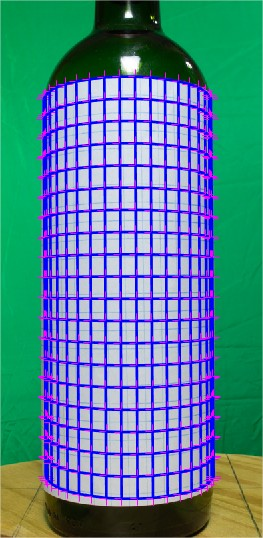
\includegraphics[width=.4\linewidth]{TCC/Imagens/ensaios/a_2020.jpg} 
            &
            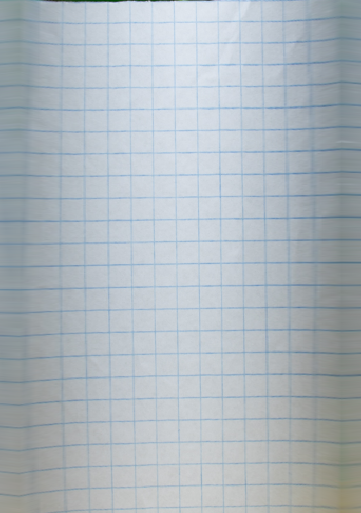
\includegraphics[width=.55\linewidth]{TCC/Imagens/ensaios/b_2020.png}
            \\
            (a) Imagem original & (b) Imagem planificada.
            \end{tabular}
        \fonte{O autor (2020).}
	\end{minipage}
    \label{fig:ensaio_2_2020a}
\end{figure}

\begin{figure}[ht]
    \caption{Resultado da planificação com N = 30.}     
    \centering
    \vspace{0.3cm}
    \begin{minipage}{.5\textwidth}
      \centering
            \begin{tabular}{cc}
            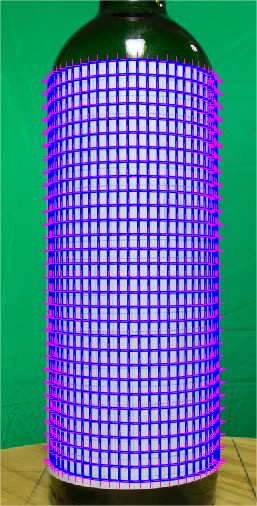
\includegraphics[width=.4\linewidth]{TCC/Imagens/ensaios/a_3030.jpg} 
            &
            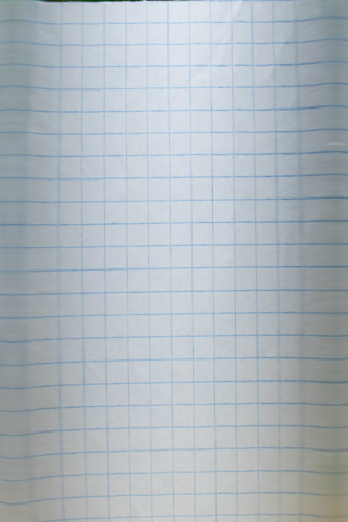
\includegraphics[width=.55\linewidth]{TCC/Imagens/ensaios/b_3030.png}
            \\
            (a) Imagem original & (b) Imagem planificada.
            \end{tabular}
        \fonte{O autor (2020).}
	\end{minipage}
    \label{fig:ensaio_2_3030a}
\end{figure}


Como mencionado, a utilização de uma maior quantidade de pontos de referência sobre a imagem resulta em um acréscimo significativo no custo computacional. 
Para realizar a medição de tempo necessário para cada execução, foi utilizada a ferramenta \textit{Profile} do MATLAB\textsuperscript{\tiny\textregistered}, que retorna a demanda de tempo em segundos de acordo com a utilização de cada método executado no código. Os valores de tempo analisados se atribuem somente ao método de planificação da imagem, desconsiderando o tempo de redimensionamento da imagem, tempo de alocação, etc. No gráfico disposto na Figura~\ref{fig:grafico_time} é demonstrado o tempo de execução do método de compensação das imagens de acordo com a quantidade de pontos.

\begin{figure}[ht]
    \caption{Tempo de execução (em segundos) para a quantidade de pontos total atribuída.}
    \centering
    \vspace{.3cm}
    \begin{minipage}{.7\textwidth}
        \hspace{.3cm}
        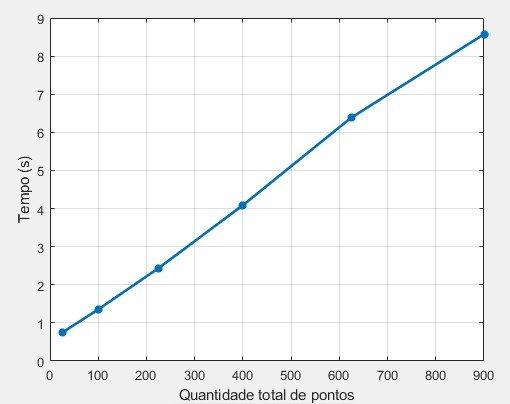
\includegraphics[width=\textwidth]{TCC/Imagens/ensaios/grafico.jpg}
        \fonte{O autor (2020).}
	\end{minipage}
    \label{fig:grafico_time}
\end{figure}

Observando-se o gráfico é possível afirmar que o tempo de execução cresce linearmente de acordo com o número de pontos atribuídos. A obtenção desses valores foi realizada seguindo as regras: execução de cinco realizações do algoritmo para cada valor de $N$, sendo considerada a média  dos valores de cada realização como o valor utilizado no gráfico; em cada uma das execuções, o comando \textit{clear all} era utilizado, a fim de evitar toda a pré-alocação de memória e outros fatores utilizados pela ferramenta para melhorar seu desempenho.

\section{Montagem da Panorâmica}

Nesta seção é avaliada a montagem da panorâmica considerando o movimento conhecido da garrafa. Como mencionado, esse sistema considera que a cena é espacialmente estática, ou seja, a garrafa e a câmera sempre vão estar fixas, realizando apenas o movimento de rotação 
da garrafa. A Figura~\ref{fig:panoramica} demonstra o resultado da montagem da panorâmica formada a partir das figuras dispostas em Figura~\ref{fig:figs_panoramica} (ver anexo A).

\begin{figure}[ht]
    \caption{Resultado da panorâmica cortando 45$^\circ$.}
    \centering
    \vspace{.3cm}
    \begin{minipage}{\textwidth}
    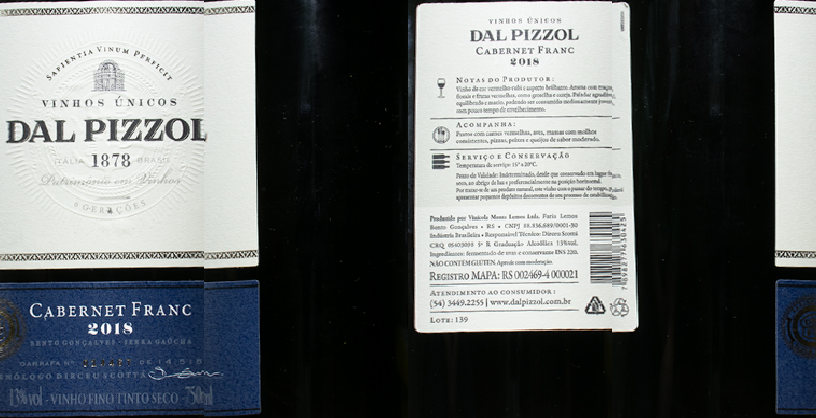
\includegraphics[width=\textwidth]{TCC/Imagens/result_45.png}
        \fonte{O autor (2020).}
	\end{minipage}
    \label{fig:panoramica}
\end{figure}

Cabe ressaltar a importância da precisão do sistema mecânico que compõe a solução proposta sistema. Visto que o local de costura do mosaico é facilmente identificável pelos diferentes níveis de iluminação nas imagens, para comentar os detalhes, cada quarto de imagem será nomeado como A, B, C e D, respectivamente. Nota-se pelas  regiões 
B e C que existe uma leve inclinação vertical no ponto de apoio da garrafa, o que interfere diretamente no alinhamento do sistema, que considera o posicionamento da garrafa como confiavelmente fixo, ou seja, quanto maior for o nível de controle do sistema mecânico, melhores podem ser os resultados obtidos através do método.

Neste resultado também é possível analisar que a desconsideração de 45º (1/4) em ambos os lados de cada imagem, apesar de terem sido utilizados valores teórico e ideais para o dimensionado aqui apresentado, resultou em uma boa representação de ponto de costura entre as imagens. Isto pode visto na junção do ''L'' (''em Pizzol''), bem como a extensão legível na parte inferior da costura entre os segmentos de imagem A e B.

Considerando que o presente trabalho conta com diversas ''não-idealidades'' para a implementação, o método conseguiu demonstrar através de uma única imagem todo o perímetro da garrafa, mesmo que com algumas falhas. Supondo um sistema mecânico superior em níveis de precisão, bem como o conhecimento dos principais
parâmetros da câmera que está sendo utilizada, os resultados de montagem da panorâmica podem ser melhorados a fim de corrigir pequenas imperfeições.



\chapter{Considerações finais}

Neste trabalho foi proposta uma etapa de um sistema computacional responsável por inspecionar rótulos de envazados com formato essencialmente cilíndricos. Aqui, se tratou do problema a partir do ponto de vista do processamento de imagens, com o propósito de corrigir as distorções causadas pelo formato do objeto quando reproduzido no plano do sensor da câmera, bem como a formação de uma panorâmica que abrange todo o perímetro do objeto.

Como o sistema proposto utiliza somente uma câmera física, emulando as outras três com translações do objeto (com passos angulares de 90$^\circ$) a fim de capturar a informação de todo o perímetro da garrafa, assume-se que o ponto no espaço ocupado pela garrafa é o mesmo nas quatro fotografias consideradas na composição da panorâmica. 

As distorções provenientes ao formato do objeto (cilíndrico) são mapeadas através das equações \eqref{equacao:dist_horz} e \eqref{equacao:dist_vert} a partir da variação angular do sistema de coordenadas da imagem. O sistema negligencia distorções provenientes da lente da câmera, sendo esse um fator que pode ser implementado em trabalhos futuros. A calibração desse parâmetro permite um dimensionamento melhor da representação angular real de cada uma das fotografias, auxiliando na montagem do mosaico. Também é importante destacar que o mapeamento proposto por \cite{Lin:2013} exige uma confiança mecânica do sistema de aquisição que, apesar de ser minucioso, não é um grande problema para aplicações industriais.

As compensações geométricas do sistema são realizadas através da seleção de quatro coordenadas (formando um paralelogramo) provenientes ao mapeamento, sendo estes submetidos a uma transformação geométrica projetiva, mudando seu formato para um retângulo. A realização desta operação com todos os pontos do mapa forma uma nova imagem planificada do rótulo.

Por fim, as quatro imagens retificadas são submetidas ao processo de montagem do mosaico. Este, apesar de depender de um sistema mecânico robusto e confiável, se demonstrou minimamente eficiente a ponto de permitir um ponto ideal de costura aceitável para uma inspeção menos delicada.

Trabalhos futuros  também podem ser realizados na direção de avaliar uma figura de mérito adequada para a  comparação de diferentes panorâmicas. Resultados preliminares indicam que as altas frequências das panorâmicas obtidas podem ser suficientes para a avaliação do correto (ou não) posicionamento do rótulo da garrafa, através da comparação com um padrão.

%para incluir a delimitação automática do rótulo analisado através de uma rede neural e/ou segmentação por formas, por exemplo. Com uma calibração da câmera é possível encontrar o ponto máximo de visão alcançado, dimensionando da representação angular de cada uma das imagens com maior precisão. Além disso, há espaços para melhoria no desempenho do sistema; visando a utilização em de tempo real, poderia ser empregado no algoritmo ferramentas de computação paralela/concorrente a fim de propor um processamento mais rápido das imagens.


%=======================================================================
% Referências
%=======================================================================
\bibliography{bibliografia}
\annex
\chapter{\hspace{1.2cm}Montagem da panorâmica}

\begin{figure}[ht]
    \caption{Imagens utilizadas para a formação da panorâmica.}     
    \centering
    \vspace{0.3cm}
    \begin{minipage}{.9\textwidth}
      \centering
      \begin{tabular}{cc}
            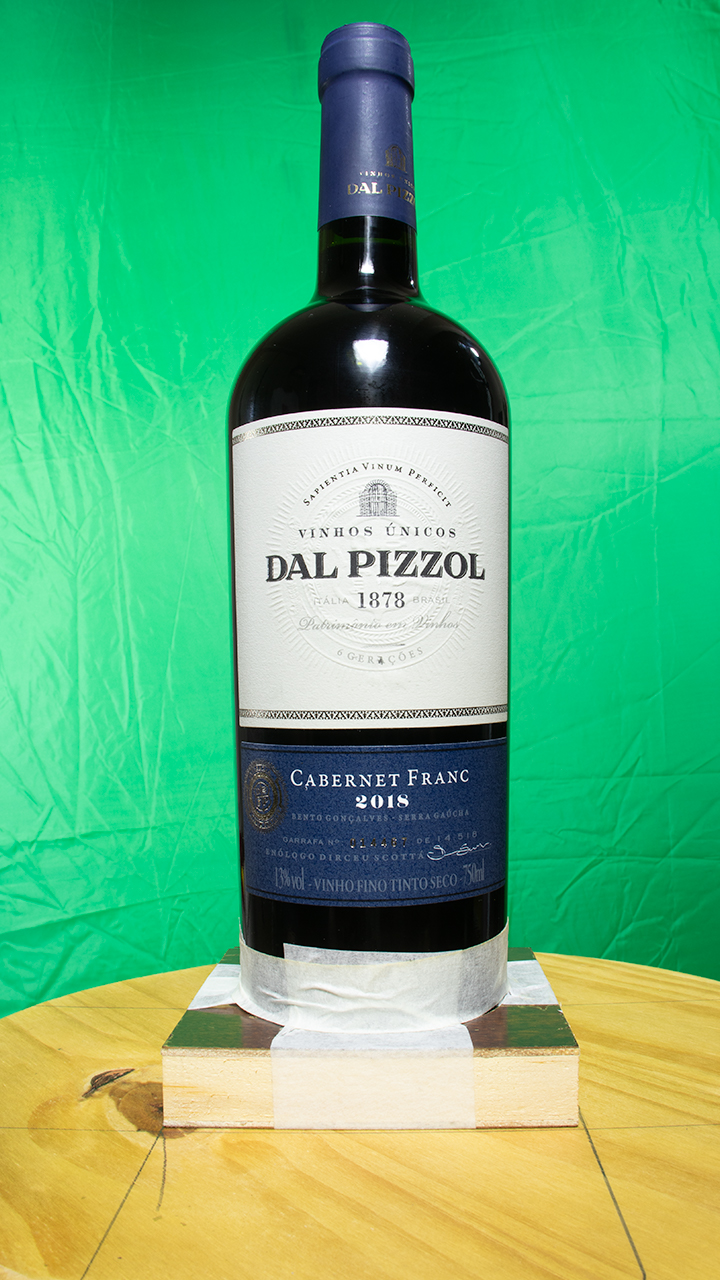
\includegraphics[width=.3\textwidth]{TCC/Imagens/ensaios/0.jpg} 
            &
            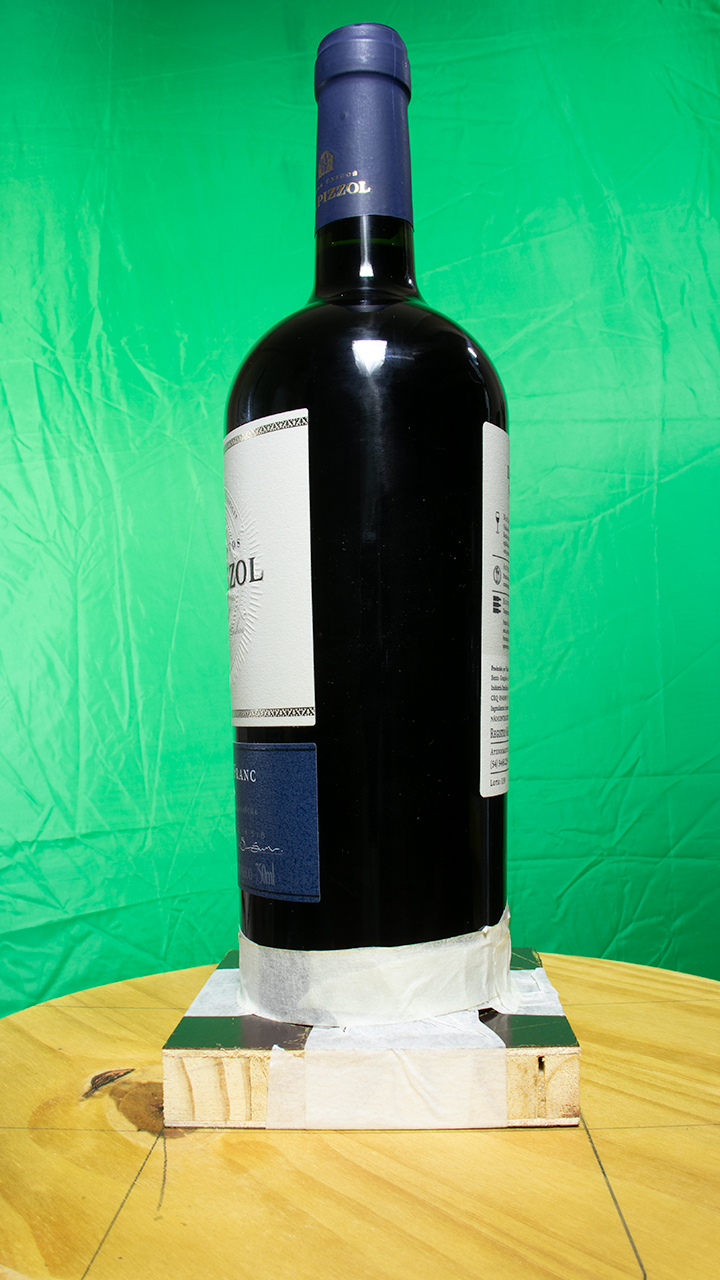
\includegraphics[width=.3\textwidth]{TCC/Imagens/ensaios/90.jpg} \\
            (a) & (b)\\
            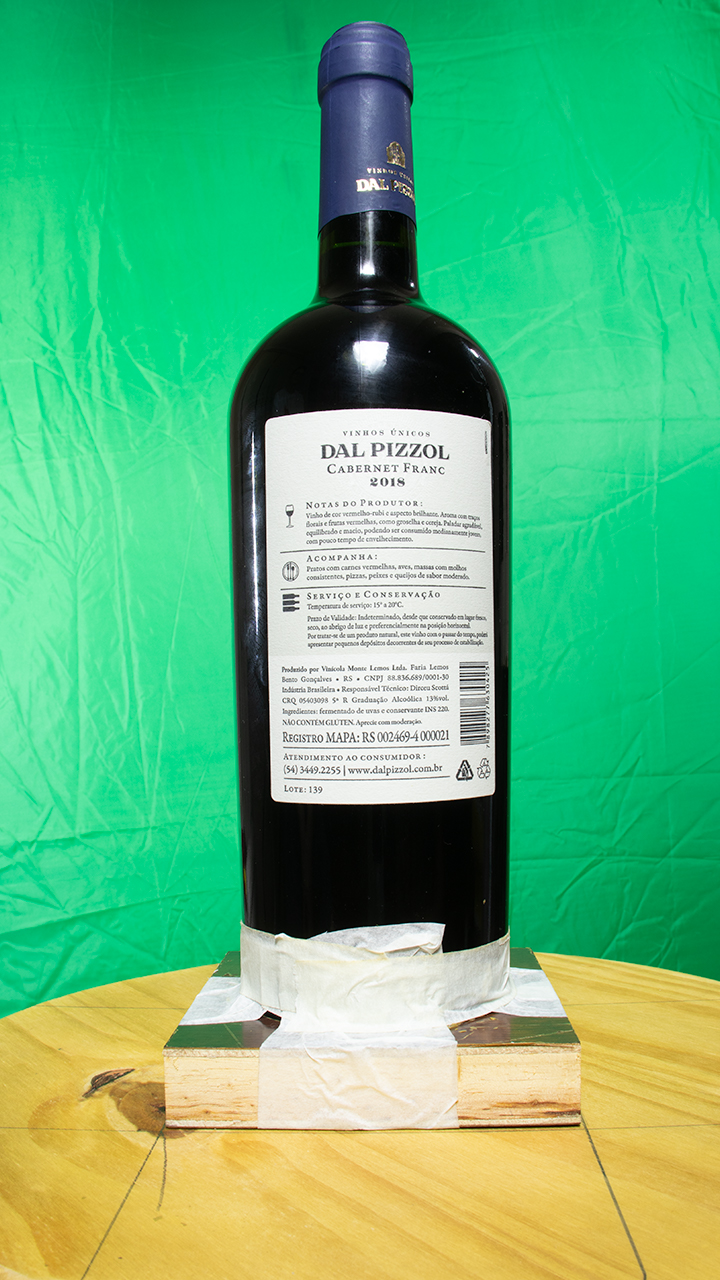
\includegraphics[width=.3\textwidth]{TCC/Imagens/ensaios/180.jpg} 
            &
            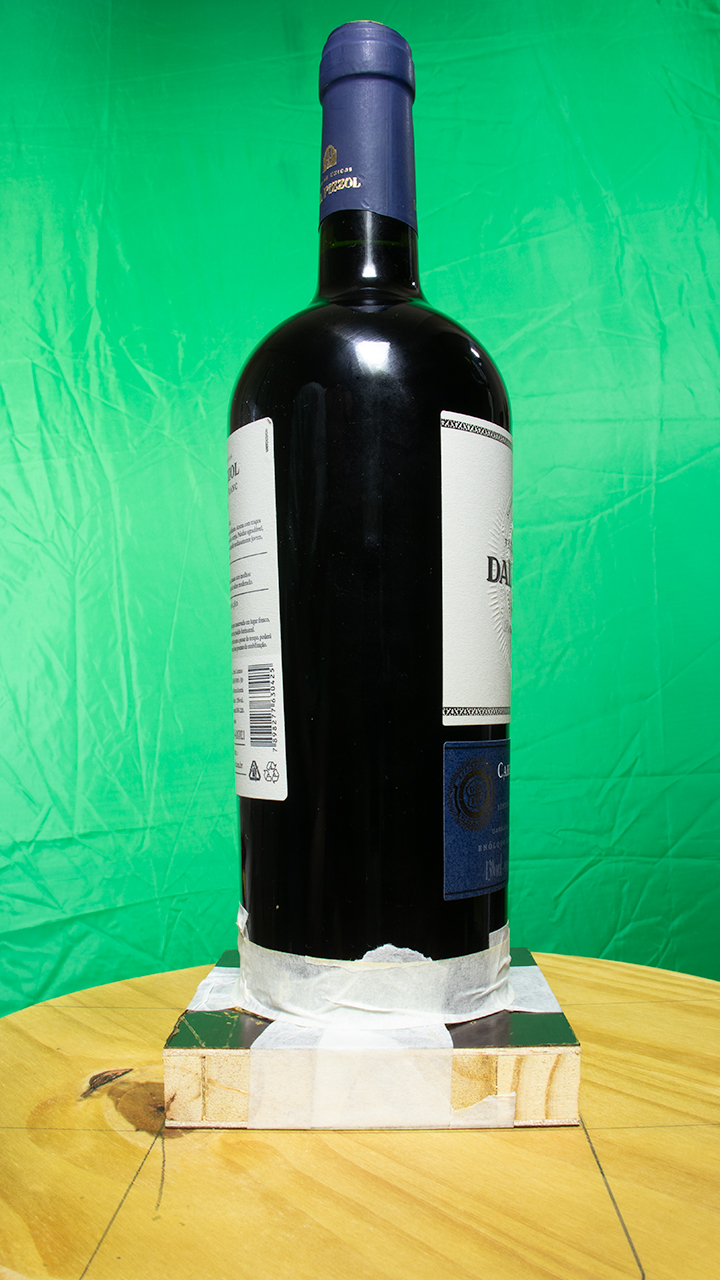
\includegraphics[width=.3\textwidth]{TCC/Imagens/ensaios/270.jpg} \\
            (c) & (d)
            \end{tabular}
            \fonte{O autor, 2020.}
	\end{minipage}
    \label{fig:figs_panoramica}
\end{figure}

% \begin{figure}[ht]
%     \label{fig:figs_panoramica}
%     \centering
%     \caption{Imagens utilizadas para a formação da panorâmica}
%     \vspace{.2cm}
%     \begin{tabular}{cc}
%     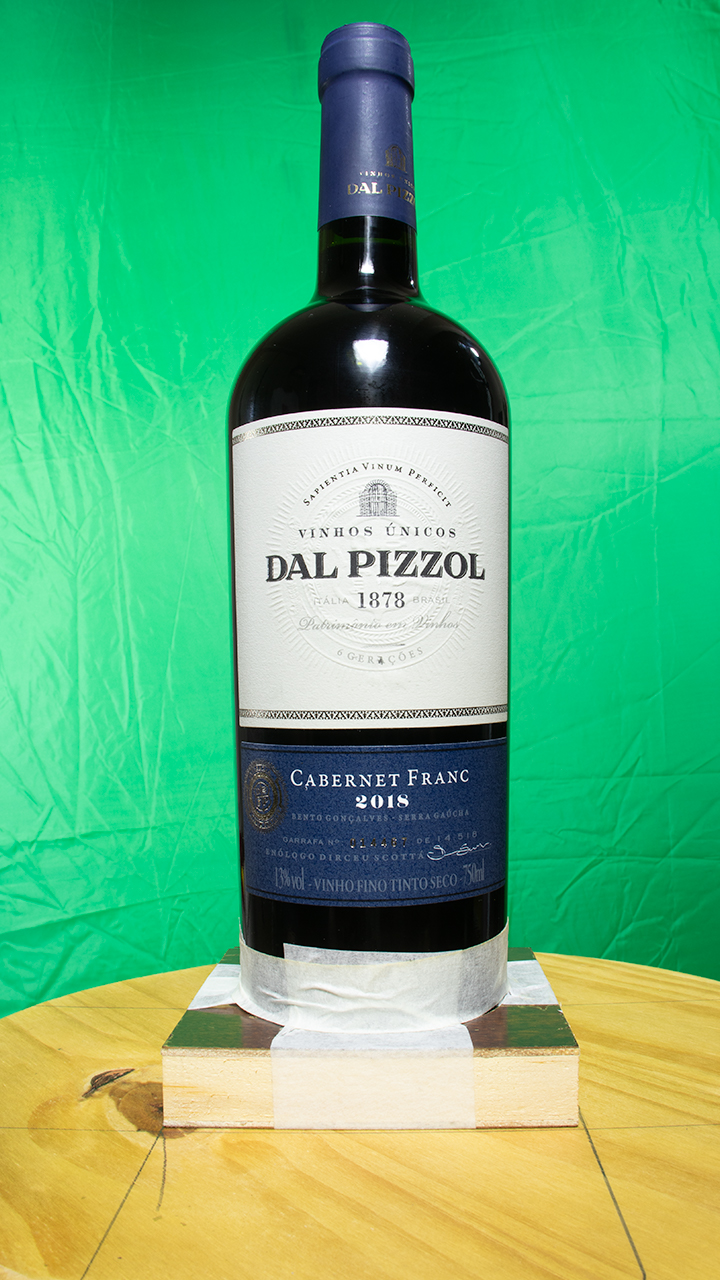
\includegraphics[width=.3\linewidth]{TCC/Imagens/ensaios/0.jpg} 
%     &
%     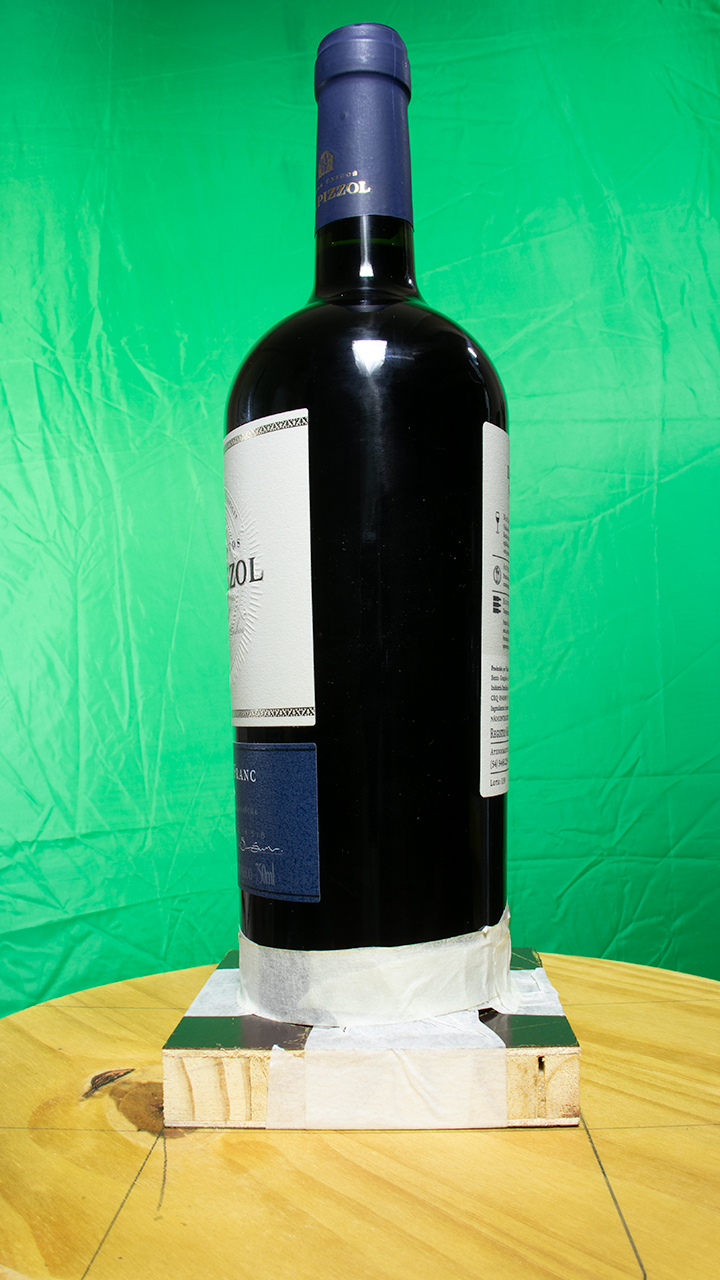
\includegraphics[width=.3\linewidth]{TCC/Imagens/ensaios/90.jpg} \\
%     (a) & (b)\\
%     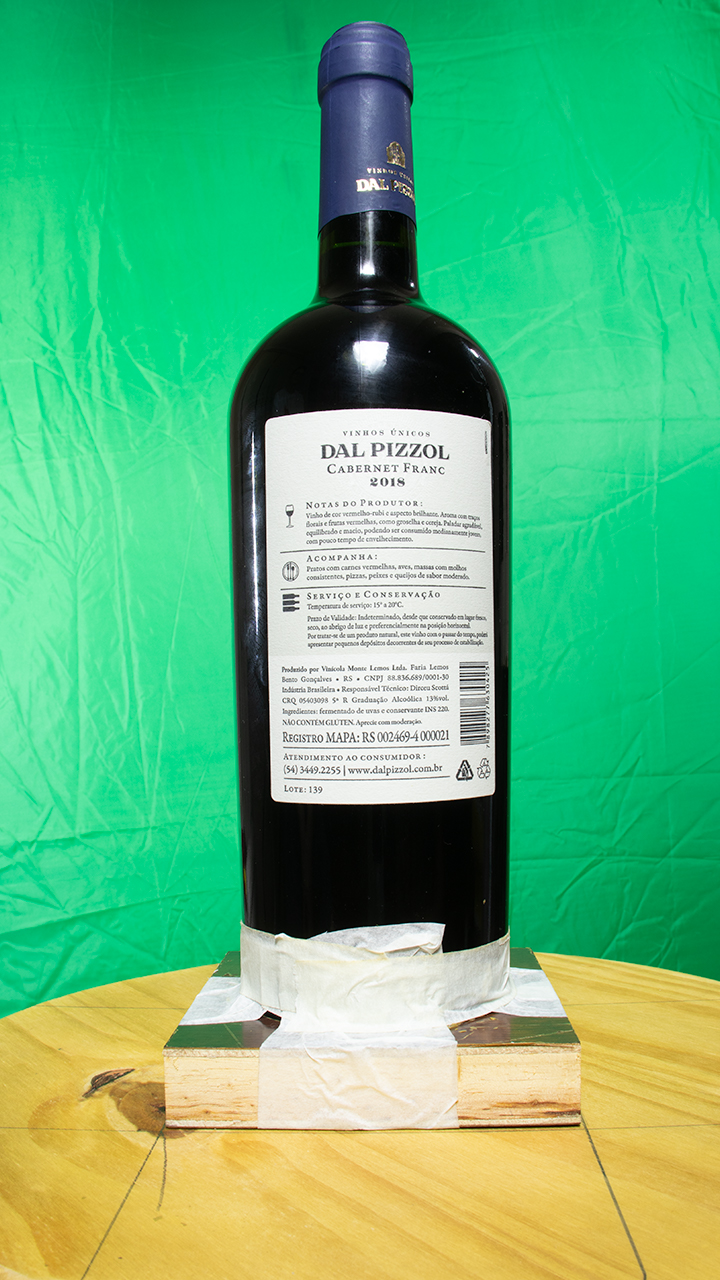
\includegraphics[width=.3\linewidth]{TCC/Imagens/ensaios/180.jpg} 
%     &
%     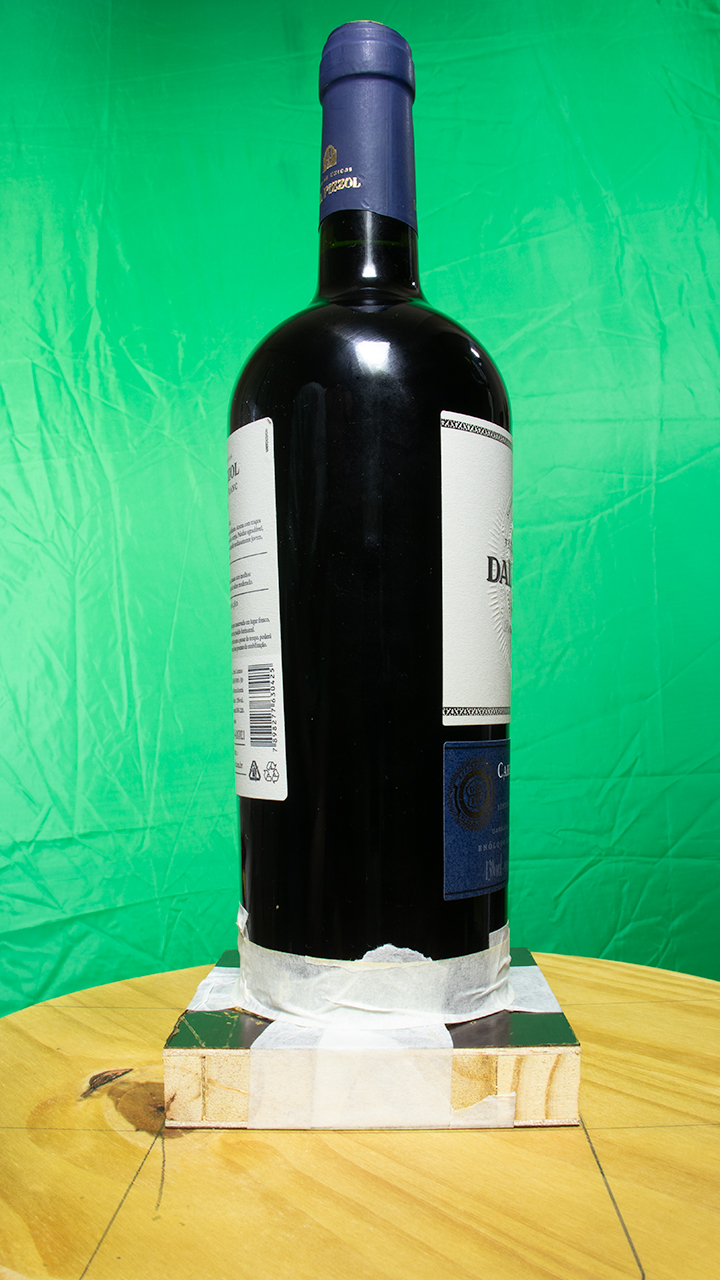
\includegraphics[width=.3\linewidth]{TCC/Imagens/ensaios/270.jpg} \\
%     (c) & (d)
%     \end{tabular}
%     \fonte{O autor, 2020.}    
% \end{figure}


    


\end{document}
